%%%%%%%% Local Spectral Clustering of Density Upper Level Sets %%%%%%%%%%%%%%%%%

\documentclass{article}
\usepackage{microtype}
\usepackage{graphicx}
\usepackage{float}
\usepackage[export]{adjustbox}
\usepackage{subcaption}
\usepackage{booktabs}
\usepackage{xcolor}
\usepackage{xr-hyper}
\usepackage{hyperref}
\usepackage[reqno]{amsmath}
\usepackage{amsfonts, amsthm, amssymb}
\usepackage{algorithm}
\usepackage{algorithmic}
\usepackage[parfill]{parskip}
\usepackage{enumerate}
\usepackage[shortlabels]{enumitem}
\usepackage{bm}
\usepackage{fullpage}

\usepackage[square,sort,comma,numbers]{natbib}
\renewcommand{\bibname}{REFERENCES}
\renewcommand{\bibsection}{\subsubsection*{\bibname}}

% Left and right equations
\makeatletter
\newcommand{\leqnomode}{\tagsleft@true\let\veqno\@@leqno}
\newcommand{\reqnomode}{\tagsleft@false\let\veqno\@@eqno}
\makeatother


\newcommand{\diam}{\mathrm{diam}}
\newcommand{\set}[1]{\left\{#1\right\}}
\newcommand{\defeq}{\overset{\mathrm{def}}{=}}
\newcommand{\vol}{\mathrm{vol}}
\newcommand{\cut}{\mathrm{cut}}
\newcommand{\abs}[1]{\left \lvert #1 \right \rvert}
\newcommand{\N}{\mathbb{N}}
\newcommand{\Reals}{\mathbb{R}}
\newcommand{\Rd}{\Reals^d}
\newcommand{\norm}[1]{\left\lVert#1\right\rVert}
\newcommand{\1}{\mathbf{1}}
\newcommand{\Phibf}{\mathbf{\Phi}}
\newcommand{\Psibf}{\mathbf{\Psi}}
\newcommand{\dist}{\mathrm{dist}}

%%% Vectors
\newcommand{\pbf}{\mathbf{p}}
\newcommand{\qbf}{\mathbf{q}}
\newcommand{\ebf}[1]{\mathbf{e}_{#1}}
\newcommand{\pibf}{\bm{\pi}}

%%% Matrices
\newcommand{\Abf}{\mathbf{A}}
\newcommand{\Xbf}{\mathbf{X}}
\newcommand{\Wbf}{\mathbf{W}}
\newcommand{\Lbf}{\mathbf{L}}
\newcommand{\Dbf}{\mathbf{D}}
\newcommand{\Ibf}[1]{\mathbf{I}_{#1}}

%%% Probability distributions (and related items)
\newcommand{\Pbb}{\mathbb{P}}
\newcommand{\Cbb}{\mathbb{C}}

%%% Sets
\newcommand{\Cset}{\mathcal{C}}
\newcommand{\Aset}{\mathcal{A}}
\newcommand{\Asig}{\Aset_{\sigma}}
\newcommand{\Csig}{\Cset_{\sigma}}

%%% Operators
\DeclareMathOperator*{\argmin}{arg\,min}

%%% Algorithm notation
\newcommand{\ppr}{{\sc PPR}}
\newcommand{\pprspace}{{\sc PPR~}}

\newtheoremstyle{aldenthm}
{6pt} % Space above
{6pt} % Space below
{\itshape} % Body font
{} % Indent amount
{\bfseries} % Theorem head font
{.} % Punctuation after theorem head
{.5em} % Space after theorem head
{} % Theorem head spec (can be left empty, meaning `normal')

\theoremstyle{aldenthm}
\newtheorem{theorem}{Theorem}
\newtheorem{definition}{Definition}
\newtheorem{lemma}{Lemma}
\newtheorem{corollary}{Corollary}

\newtheoremstyle{aldenrmrk}
{6pt} % Space above
{6pt} % Space below
{} % Body font
{} % Indent amount
{\itshape} % Theorem head font
{.} % Punctuation after theorem head
{.5em} % Space after theorem head
{} % Theorem head spec (can be left empty, meaning `normal')

\theoremstyle{aldenrmrk}
\newtheorem{remark}{Remark}

\begin{document}

\title{Local Spectral Clustering of Density Upper Level Sets}
\author{Alden Green, Sivaraman Balakrishnan, and Ryan Tibshirani}
\date{\today}
\maketitle

\begin{abstract}
\vskip 0.1 in % RESOLVED
Spectral clustering methods are a family of popular nonparametric clustering
tools.  Recent works have proposed and analyzed \emph{local} spectral methods,
which extract clusters using locally-biased random walks around a user-specified
seed node.  Several authors have shown that local methods, such as personalized
PageRank (PPR), have worst-case guarantees for certain graph-based measures of
cluster quality.  In contrast to existing works, we analyze PPR in a traditional
statistical learning setup, where we obtain samples from an unknown
distribution, and aim to identify connected regions of high-density (density
clusters).  We introduce two natural criteria for cluster quality, and derive
bounds for these criteria when evaluated on empirical analogues of density
clusters. Moreover, we prove that PPR, run on a neighborhood graph, extracts
sufficiently salient density clusters.
\end{abstract}

\section{Introduction}
\label{sec: introduction}

Let $\mathbf{X} = \{x_1, \ldots, x_n\}$ be a sample drawn i.i.d.\ from a
distribution $\Pbb$ on $\Rd$, with density $f$, and consider the problem of 
clustering: splitting the data into groups which satisfy some notion of
within-group similarity and between-group difference.  We focus on spectral
clustering methods, a family of powerful nonparametric clustering algorithms.
Roughly speaking, a spectral technique first constructs a geometric graph $G$,
where vertices are associated with samples, and edges correspond to proximities
between samples. It then learns a feature embedding based on the Laplacian of
$G$, and applies a simple clustering technique (such as k-means clustering) in
the embedded feature space.

To be more precise, let $G=(V,E,w)$ denote a weighted, undirected graph  
constructed from the samples $\mathbf{X}$, where $V=\{1,\ldots,n\}$, and $w_{uv}
= K(x_u,x_v) \geq 0$ for $u,v \in V$, and a particular kernel function $K$.
Here $(u,v) \in E$ if and only if $w_{uv} > 0$.  We denote by $\Abf \in
\Reals^{n \times n}$ the weighted adjacency matrix, which has entries
$A_{uv}=w_{uv}$, and by $\Dbf$ the degree matrix, with 
\smash{$\Dbf_{uu} = \sum_{v \in V} \Abf_{uv}$}.  We also denote by $\Wbf,\Lbf$
the random walk transition probability matrix and normalized\footnote{Other
  popular choices here include the unnormalized Laplacian, and symmetric
  normalized Laplacian.} 
Laplacian matrix, respectively, which are defined as
$$
\Wbf = \Dbf^{-1}\Abf, \quad \Lbf = \Ibf{} - \Wbf,
$$
where $\Ibf{} \in \Reals^{n\times n}$ is the identity matrix.  Classical global
spectral methods take a eigendecomposition $L=U \Sigma U^T$, use some 
number of eigenvectors (columns in $U$) as a feature representation for the
samples, and then run (say) k-means in this new feature space.

When applied to geometric graphs constructed from a large number of samples,
global spectral clustering methods can be computationally cumbersome and   
insensitive to the local geometry of the underlying distribution
\citep{leskovec2010,mahoney2012}.  This has led to recent increased interest in
local spectral algorithms, which leverage locally-biased spectra computed using
random walks around a user-specified seed node.  A popular local clustering
algorithm is Personalized PageRank (PPR), first introduced by
\citep{haveliwala2003}, and further developed by
\citep{spielman2011,spielman2014,andersen2006,mahoney2012,zhu2013},
among others.  

Local spectral clustering techinques have been practically very successful
\citep{leskovec2010,andersen2012,gleich2012,mahoney2012,wu2012}, which has led
many authors to develop supporting theory
\citep{spielman2013,andersen2009,gharan2012,zhu2013} that gives worst-case
guarantees on traditional graph-theoretic notions of cluster quality (like
conductance).  In this paper, we adopt a more traditional statistical viewpoint,
and examine what the output of a local clustering algorithm on $\Xbf$ reveals
about the unknown density $f$.  In particular, we examine the ability of the PPR
algorithm to recover \emph{density clusters} of $f$, which are defined as the
connected components of the upper level set $\{x \in \Rd : f(x) \geq \lambda\}$
for some threshold $\lambda > 0$ (a central object of central interest in the
classical statistical literature on clustering, dating back to
\citet{hartigan1981}).

\subsection{Graph Connectivity Criteria}

Here we define a pair of criteria that reflect the quality of a cluster with
respect to $G=(V,E,w)$.  There are many graph-based measures of cluster quality  
that one could consider; see, e.g., \citep{yang2015,fortunato2010} for 
an overview.  The pair of criteria that we focus on are (arguably) quite
natural, and moreover, they play a fundamental role in our analysis 
of the PPR algorithm.  Our two criteria capture the \emph{external} and
\emph{internal} connectivity of a subset $S \subseteq V$, denoted $\Phi(S; G)$
and $\Psi(S; G)$, respectively, and defined below in turn.  

\paragraph{External Connectivity: Normalized Cut}

Define the cut between subsets $S,S' \subseteq V$ to be
$$
\cut(S, S'; G) = \sum_{u \in S} \sum_{v \in S'} w_{uv},
$$
and define
\smash{$\vol(S; G) = \cut(S, V; G) = \sum_{u \in S} \sum_{v \in V} w_{uv}$}.  
As our notion of external connectivity, we use the \emph{normalized cut}  
of $S$, defined as 
\begin{equation}
\label{eqn: norm_cut}
\Phi(S; G) = \frac{\cut(S; G)}{\min\{\vol(S; G), \vol(S^c; G)\}},
\end{equation} 
where we abbreviate $\cut(S; G) = \cut(S; S^c; G)$.

\paragraph{Internal Connectivity: Inverse Mixing Time}

For $S \subseteq V$, denote by $G[S] = (S, E_S, w_S)$ the subgraph induced by 
$S$ (where the edges are $E_S = E \cap (S \times S)$). Let $\Abf_S,\Dbf_S$
be the adjacency matrix and degree matrix, respectively, of $G[S]$.  Define the
random walk matrix as usual, $\Wbf = \Dbf_S^{-1} \Abf_S$, and for $v \in V$,
write 
$$
q_{vu}^{(t)} = e_v\Wbf_S^t e_u
$$
for the $t$-step transition probability of a random walk over $G[S]$
originating at $v$.\footnote{Given a starting node $v$ and and a random walk
  defined by transition probability matrix $\mathbf{P}$, the notation $e_v
  \mathbf{P}^t$ is used to denote the distribution of the random walk after $t$
  steps.}   Also write \smash{$\widetilde\pibf = (\widetilde\pi_{u})_{u \in S}$}
for the stationary distribution of this random walk.  (Given the definition of 
$\Wbf_S$, it is well-known that the stationary distribution is given by
\smash{$\widetilde\pi_{u} = (\Dbf_{S})_{uu} / \vol(S; G[S])$}.) 

Our internal connectivity parameter will capture the time it takes for the
random walk over $G[S]$ to mix (approach the stationary distribution)
uniformly over $S$.  For this, we first define the \emph{relative pointwise mixing
  time} of $G[S]$ as 
$$
\tau_{\infty}(G[S]) = \min\set{ m: \frac{|q_{vu}^{(m)} - 
      \widetilde\pi_u|}{\widetilde\pi_u} \leq \frac{1}{4}, 
    \; \text{for $u,v \in V$}}. 
$$
%where \smash{$\qbf = (\qbf_v^{(1)}, \qbf_v^{(2)}, ...)_{v \in V}$}, and
%\smash{$\qbf_v^{(m)} = (q_{vu}^{(m)})_{u \in V}$}. 
% RJT: I got rid of the notational dependence on \qbf, because these quantities
% are in turn just defined in terms of the induced subgraph G[S]
% AJG: RESOLVED
Now our internal connectivity parameter is simply the inverse mixing time, 
\begin{equation}
\label{eqn: inv_mixing_time}
\Psi(S; G) = \frac{1}{\tau_{\infty}(G[S])}.
\end{equation}

If $S$ has normalized cut no greater than $\Phi$, and inverse mixing time no
less than $\Psi$, we call it as a \emph{$(\Phi,\Psi)$-cluster}. Both
local \citep{zhu2013} and global \citep{kannan04} spectral algorithms have been
shown to output clusters (or partitions) which approximate the optimal $(\Phi,
\Psi)$-cluster (or partition) for a given graph $G$.\footnote{In the case of
  \citep{kannan04}, the internal connectivity parameter $\phi$ is actually the
  conductance, i.e., the minimum normalized cut within the subgraph $G[S]$. See
  Theorem 3.1 in their paper for details; however, note that $\phi^2 /
  \log(\vol(S)) \leq O(\Psi)$, and so the lower bound on $\phi$ translates to a
  lower bound on $\Psi$.}   

\subsection{PPR on a Neighborhood Graph}

We now describe the clustering algorithm that will be our focus for the rest of 
the paper. We start with the geometric graph that we form based on the samples 
$\Xbf$: for a radius $r > 0$, we consider the \emph{$r$-neighborhood graph} of 
$\Xbf$, denoted $G_{n,r}=(V,E)$, an unweighted graph with vertices
$V=\{1,\ldots,n\}$, and an edge $(u,v) \in E$ if and only if $\norm{x_u - x_v}
\leq  r$, where $\norm{\cdot}$ denotes Euclidean norm.  Note that this is a
special case of the general construction introduced above, with 
$K(u,v) = 1(\norm{x_u - x_v} \leq r)$. 

Next, we define the PPR vector $\pbf = \pbf(v,\alpha;G_{n,r})$, with respect to  
a seed node $v \in V$ and a teleportation parameter $\alpha \in [0,1]$, to be
the solution of the following linear system:
\begin{equation}
\label{eqn: ppr_vector}
\pbf = \alpha \ebf{v} + (1 - \alpha) \pbf \Wbf,
\end{equation}
where $\Wbf$ is the random walk matrix of the underlying graph $G_{n,r}$ 
and $e_{v}$ denotes indicator vector for node $v$ (with a 1 in the $v$th
position and 0 elsewhere).  In practice, we can approximately solve the above
linear system via a simple, efficient random walk, with appropriate restarts to
$v$. 

For a level $\beta > 0$ and a target volume $\vol_0 > 0$, we define a
\emph{$\beta$-sweep cut} of $\pbf$ as  
\begin{equation}
\label{eqn: sweep_cuts}
S_\beta = \{u \in V: \textcolor{red}{\frac{p_u}{\Dbf_{uu}}} > \frac{\beta}{\vol_{0}}\}.
\end{equation}
Having computed sweep cuts over a range \smash{$\beta \in  
(\frac{1}{40},\frac{1}{11})$},\footnote{The choice of a specific range such as 
\smash{$(\frac{1}{40}, \frac{1}{11})$} is standard in the analysis of PPR
algorithms, see, e.g., \citep{zhu2013}.}
we output a cluster \smash{$\widehat{C} = S_{\beta^*}$}, based on the sweep cut
$S_{\beta^*}$ that minimizes the normalized cut \smash{$\Phi(S_{\beta^*};
  G_{n,r})$} as defined in \eqref{eqn: norm_cut}. For concreteness, we summarize
this procedure in Algorithm \ref{alg: ppr}.   

\begin{algorithm}
\caption{PPR on a Neighborhood Graph}
\label{alg: ppr}	
{\bfseries Input:} data $\Xbf=\{x_1,\ldots,x_n\}$, radius $r > 0$, teleportation 
parameter $\alpha \in [0,1]$, seed $v \in \Xbf$, target stationary volume $\pi_0 >
0$. \\   
{\bfseries Output:} cluster $\widehat{C} \subseteq V$.
\begin{algorithmic}[1]
  \STATE Form the neighborhood graph $G_{n,r}$.
  \STATE Compute the PPR vector $\pbf(v, \alpha; G_{n,r})$ as in \eqref{eqn:
    ppr_vector}. 
  \STATE For $\beta \in (\frac{1}{40}, \frac{1}{11})$ compute sweep cuts
  $S_{\beta}$ as in \eqref{eqn: sweep_cuts}.
  \STATE Return \smash{$\widehat{C} = S_{\beta^*}$}, where 
  $$
  \beta^* = \argmin_{\beta \in (\frac{1}{40}, \frac{1}{11})} \Phi(S_{\beta}; G_{n,r}).
  $$
\end{algorithmic}
\end{algorithm}

\subsection{Summary of Results}

% It is worth calling attention to some other work on computing the normalized
% cut over neighborhood graphs. In this context, continuous analogues to (for
% instance) normalized cut have been defined, over the data-manifold rather than
% the graph, and convergence finite sample graph-theoretic functionals to their
% continuous counterparts has been shown 
% \cite{garciatrillos16, arias-castro12, maier11}. 
% However, in addition to the graph-minimization problem being computationally
% infeasible, these continuous analogues are not always easily interpretable --
% and their corresponding minimizers not always easily identifiable -- for the
% particular density function under consideration. Of course, relating these
% partitions to the arguably more simply defined high density clusters can be
% also challenging in general. Intuitively, however, under the right conditions
% such high-density clusters should have more edges within themselves than to
% the remainder of the graph. We formalize this intuition next. 

%% RJT: I didn't know where to put this.  It was out of place, and now I'm not
%% sure where it goes ... should it go in related work?

%It is worth pointing out that in this context, some theory has been developed
%regarding how graph theoretic quantities such as the normalized cut $\Phi$ (and
%others) relate to properties of the underlying distribution $f$ as well as the
%kernel function $k$. Such analyses typically proceed by defining a continuous
%analogue to the measure of cluster quality under consideration. Then, under
%appropriate specification of $k$ and a proper schedule of $(r_n)$, convergence
%of clusters output by spectral (and other) algorithms to the corresponding
%minima of these continuous analogues has been shown \cite{vonluxburg2008,
%garciatrillos18}. 

%% RJT: This was already commented out before

Let $\Cbb_f(\lambda)$ denote the connected components of the density upper level
set $\{x \in \Rd: f(x) > \lambda\}$.  For a given density cluster $\Cset \in
\Cbb_f(\lambda)$, we call $\Cset[\Xbf] = \Cset \cap \Xbf$ the \emph{empirical
density cluster}. Below we give two notions of performance of a density cluster estimate. 

\begin{definition}[Misclassification rate]
\label{def: misclassification_rate}
For an estimator \smash{$\widehat{\Cset} \subseteq \Xbf$} and set
$\mathcal{S} \subseteq \Reals^d$, the \emph{misclassification rate} of $\mathcal{S}$ by $\widehat{\Cset}$ is
\begin{equation}
\label{eqn: misclassification_rate}
\abs{\widehat{\Cset} \setminus (\mathcal{S} \cap \Xbf)} + \abs{(\mathcal{S} \cap \Xbf) \setminus \widehat{\Cset}}.
\end{equation}
\end{definition}    

\begin{definition}[Consistent density cluster estimation]
\label{def: consistent_density_cluster_estimation}
For an estimator \smash{$\widehat{\Cset} \subseteq \Xbf$} and cluster 
$\Cset \in \Cbb_f(\lambda)$, we say \smash{$\widehat{\Cset}$} is a consistent
estimator of $\Cset$ if for all $\Cset' \in \Cbb_f(\lambda)$ with $\Cset \not=
\Cset'$ the following holds as $n \to \infty$: 
\begin{equation}
\label{eqn: consistent_density_cluster_recovery}
\Cset[\Xbf] \subseteq \widehat{\Cset} \quad \text{and} \quad
\widehat{\Cset} \cap \Cset'[\Xbf] = \emptyset,
\end{equation}
with probability tending to 1.
\end{definition}



A summary of our main results (and outline for the rest of this paper) is as
follows.  

\begin{enumerate}
\item In Section \ref{sec: cluster_quality_bounds}, we derive in Theorem
  \ref{thm: conductance_upper_bound} an upper bound on the normalized cut of a  
  (thickened) empirical density cluster $\Csig[\Xbf]$, under natural geometric 
  conditions (precluding clusters that are arbitrarily thin).  

\item Under \textcolor{red}{largely the same set of geometric conditions}, we derive in Theorem
  \ref{thm: inverse_mixing_time_lower_bound_nonconvex} a lower bound on the
  inverse mixing time of a random walk over $\Csig[\Xbf]$.
	
\item In Section \ref{sec: consistent_cluster_estimation_with_ppr}, we show in
  Theorem \ref{thm: consistent_recovery_of_density_clusters} that the bounds on the cluster quality criteria established in Theorems \ref{thm: conductance_upper_bound} and \ref{thm:
    inverse_mixing_time_lower_bound_nonconvex} have algorithmic consequences for \ppr: 
  properly initialized, Algorithm \ref{alg: ppr} has low misclassification rate with respect to a small enlargement of the set $\Cset$, and if the density cluster $\Cset$ is particularly well-conditioned, Algorithm \ref{alg: ppr} will perform consistent density cluster estimation in the sense of \eqref{eqn: consistent_density_cluster_recovery}. 
	
\item We show in Corollary \ref{cor: appr} that these statements hold also with respect to an approximate form of \pprspace, which can be efficiently computed.

\item In Section \ref{sec: experiments}, we empirically
  demonstrate the tightness of the bounds in Theorems \ref{thm: conductance_upper_bound} and \ref{thm: inverse_mixing_time_lower_bound}, and provide examples showing how violations of the geometric conditions we require manifestly
  impact density cluster recovery by \ppr.  
\end{enumerate}

On the topic of conditions, it is worth mentioning that, as density clusters
are inherently local, focusing on the PPR algorithm actually eases our analysis
and allows us to require fewer global regularity conditions relative to those
needed for more classical global spectral algorithms.    

\subsection{Related Work}
%In addition to the background given above, a few related lines of work are worth
%highlighting. For neighborhood graphs of the type we consider, continuous analogues to (for
%instance) normalized cut have been defined, over the data-manifold rather than
%the graph, and convergence finite sample graph-theoretic functionals to their
% continuous counterparts has been shown 
% \cite{garciatrillos16, arias-castro12, maier11}. 

In addition to the background given above, a few related lines of work are worth
highlighting.
Global spectral clustering methods were first developed in the
context of graph partitioning \citep{fiedler1973,donath1973} and their
performance is well-understood in this context (see, e.g.,
\citealt{tolliver2006,luxburg2007}).  In a similar vein, several recent works
\citep{mcsherry2001,rohe2011,kamalika2012,balakrishnan2011,lei2015,abbe2018} 
have studied the efficacy of spectral methods in successfully recovering the
community structure in the stochastic block model and variants.

Building on earlier work of
\citep{koltchinskii2000}, \citep{vonluxburg2008,hein2005} studied the limiting behaviour of spectral clustering
algorithms. These authors show that when samples are obtained from a
distribution, and we appropriately construct a geometric graph, the spectrum of
the Laplacian converges to that of the Laplace-Beltrami operator on the
data-manifold. However, relating the partition obtained using the
Laplace-Beltrami operator to the more intuitively defined high-density
clusters can be challenging in general.


% AJG 4/29: I need to rewrite to explain how its similar, because
% this is a good opportunity to show that implications
% of the type given in our work are broadly of interest.

Perhaps most similar to our results are the works
\citep{vempala2004,shi2009,schiebinger2015}, who study the consistency of
spectral algorithms in recovering the latent labels in certain parametric and
nonparametric mixture models. These results focus on global rather than local
algorithms, and as such impose global rather than local conditions on the nature
of the density. Moreover, they do not in general ensure recovery of density
clusters, which is the focus in our work. 

\section{Cluster Quality Criteria Bounds for Density Clusters}  
\label{sec: cluster_quality_bounds}

\subsection{Geometric Conditions on Density Clusters}

In order to provide meaningful bounds on the normalized cut and inverse mixing
time of an empirical density cluster, we must introduce conditions on the
density $f$. Let $B(x,r) = \{y \in \Rd: \norm{y - x} \leq r\}$ be the closed
ball of radius $r > 0$, centered at $x \in \Rd$.  Given a set $\Aset
\subseteq \Rd$ and $\sigma > 0$, define $\Asig = \Aset + B(0,\sigma) = \{y \in
\Rd: \inf_{x \in \Aset} \norm{y - x} \leq \sigma\}$, which we call the
$\sigma$-expansion of $\Aset$. For a differentiable function $g: \Rd \to \Rd$, write $\nabla g(x)$ to denote the Jacobian of $g$ evaluated at $x \in \Rd$. 

We are now ready to give our required conditions, stated with respect to a density
cluster $\Cset \in \Cbb_f(\lambda)$ for some threshold $\lambda > 0$, and an
expansion parameter $\sigma > 0$. 

\begin{enumerate}[label=(A\arabic*)]
\item
\label{asmp: bounded_density}
\emph{Bounded density within cluster:} There are $0 < \lambda_{\sigma} <
\Lambda_{\sigma} < \infty$ such that
$$
\lambda_{\sigma} = \inf_{x \in \Csig} f(x) \leq \sup_{x \in \Csig} f(x) \leq
\Lambda_{\sigma}.
$$
% and 
% \begin{equation*}
% \frac{\diam \Asig}{\sigma} \leq \mu
% \end{equation*}
% where $\diam \Asig = \sup \set{d(x,y) : x,y \in \Asig}$
	
\item 
\label{asmp: low_noise_density}
\emph{Low noise density:} There exists $\gamma,c_0 > 0$ such that for all $x
\in \Rd$ with $0 < \dist(x, \Csig) \leq \sigma$,   
$$
  \inf_{x' \in \Csig} f(x') - f(x) \geq  c_0 \dist(x, \Csig)^{\gamma},
$$
where \smash{$\dist(x,\Aset) = \inf_{x_0 \in \Aset} \norm{x - x_0}$}.

\item
\label{asmp: cluster_separation}
\emph{Cluster separation:}
For all $\Cset' \in \Cbb_f(\lambda)$ with $\Cset' \not= \Cset$,
$$
\dist(\Csig,\Csig') > \sigma,
$$
where \smash{$\dist(\Aset,\Aset') = \inf_{x \in \Aset} \dist(x,\Aset')$}.  
	
\item
\label{asmp: cluster_diameter}
\emph{Cluster diameter:}
There exists $D < \infty$ such that for all $x, x' \in \Csig$,
$$
\norm{x - x'} \leq D.
$$

\item
\label{asmp: biLipschitz_mapping}
\emph{biLipschitz mapping to convex set:}
There exists $\mathcal{K} \subseteq \Rd$ convex, and $g: \Reals^d \to \Reals^d$ satisfying
\begin{equation*}
\det(\nabla g (x) ) = 1,\frac{1}{L}\norm{x - y} \leq \norm{g(x) - g(y)} \leq L \norm{x - y} ~ \text{for all $x,y \in \Reals^d$}
\end{equation*}
such that $\Csig$ is the image of $\mathcal{K}$ by $g$, $\Csig = g(\mathcal{K})$.
\end{enumerate}

Note that $\sigma$ plays several roles here, precluding arbitrarily narrow
clusters and long clusters in \ref{asmp: bounded_density} and \ref{asmp:
  cluster_diameter}, flat densities around the level set in \ref{asmp: 
  low_noise_density}, and poorly separated clusters in \ref{asmp:
  cluster_separation}. 

Assumptions \ref{asmp: bounded_density}, \ref{asmp: low_noise_density},
\ref{asmp: cluster_separation} and \ref{asmp: biLipschitz_mapping} are used to upper bound $\Phi(\Cset[\Xbf];
G_{n,r})$, whereas \ref{asmp: bounded_density}, \ref{asmp: cluster_diameter} and \ref{asmp: biLipschitz_mapping} are required to lower bound $\Psi(\Cset[\Xbf]; G_{n,r})$. We note that the
lower bound on minimum density in \ref{asmp: bounded_density} along with \ref{asmp:  
cluster_separation} are similar to the $(\sigma,\epsilon)$-saliency of
\citep{chaudhuri2010}, a standard density clustering assumption, while
\ref{asmp: low_noise_density} is seen in, e.g., \citep{singh2009} (as well as
many other works on density clustering and level set estimation.)  It is worth
highlighting that these assumptions are all local in nature, a benefit of
studying a local algorithm such as \ppr.


%%% AJG 4/29: My attempt to explain why our results aren't fatuous.

We also note that while many of these geometric conditions are typical in the density clustering literature, the restrictions we will impose upon them in order to obtain meaningful implications for \pprspace will not be. This is natural. The spectral algorithm we consider is not specifically designed for the task of level set estimation, and in fact one should expect \pprspace to fail to recover -- either in the sense of \eqref{eqn: consistent_density_cluster_recovery}, or indeed any reasonable notion of cluster recovery -- a density cluster of sufficiently large diameter or sufficiently small thickness (though we do not provide any lower bounds to this effect). Indeed, one of the primary motivations of this work was to better understand and characterize the distinctions between those level sets which are well conditioned for spectral algorithms, and those which are not.


In the next several subsections, we will derive bounds on the cluster quality
criteria evaluated on ($\sigma$-expansions of) density clusters. For notational simplicity,
hereafter for $S \subseteq V$, we will abbreviate $\Phi(S; G_{n,r})$ by
$\Phi_{n,r}(S)$, and similarly, $\Psi(S; G_{n,r})$ by $\Psi_{n,r}(S)$, and
$\tau_{\infty}(G_{n,r}[S])$ by $\tau_{n,r}(S)$. We will also use $\nu$ for
Lebesgue measure on $\Rd$, and $\nu_d = \nu(B)$ for the measure of the unit ball
$B=B(0,1)$.  

\subsection{Upper Bound on Normalized Cut}

We start with an upper bound on the normalized cut \eqref{eqn: norm_cut} of 
$\Cset_\sigma[\Xbf]$. (In Theorem \ref{thm: conductance_upper_bound}, the upper bound on the density in
Assumption \ref{asmp: bounded_density} will not actually be needed, so we omit
the parameter $\Lambda_\sigma>0$ from the theorem statement.) For $\mathcal{S} \subseteq \Reals^d$ and $r > 0$, let
\begin{equation*}
\pi_{\Pbb,r}(\mathcal{S}) := \frac{\int_{\mathcal{S}} \Pbb(B(x,r)) f(x) dx }{\int_{\Rd} \Pbb(B(x,r)) f(x) dx}.
\end{equation*}

\begin{theorem}
\label{thm: conductance_upper_bound}
Fix $\lambda > 0$, and let $\Cset \in \Cbb_f(\lambda)$ satisfy
Assumptions \ref{asmp: bounded_density}, \ref{asmp: low_noise_density},
and \ref{asmp: cluster_separation}, for some 
$\sigma, \lambda_{\sigma}, c_0, \gamma > 0$. Let $0 < r \leq \sigma/4d$ be such that
\begin{equation}
\label{eqn: weighted_cluster_volume}
\pi_{\Pbb,r}(\Csig) \leq \frac{1}{2}.
\end{equation}
 Then for any $0 < \delta < 1$, $\epsilon > 0$, if
\begin{equation}
\label{eqn: conductance_sample_complexity}
n \geq \frac{(2+\epsilon)^2\log(3/\delta)}{\epsilon^2}\left(\frac{25}
  {6 \lambda_{\sigma}^2\nu(\Csig) \nu_d r^d}\right)^2,
\end{equation}
then
\begin{equation}
  \label{eqn: conductance_additive_error_bound}
  \frac{\Phi_{n,r}(\Csig[\mathbf{X}])}{r} \leq c \frac{d}{\sigma}
  \frac{\lambda}{\lambda_{\sigma}} \frac{(\lambda_{\sigma} -
    c_0\frac{r^{\gamma}}{\gamma+1})}{\lambda_{\sigma}} + \epsilon, 
\end{equation}
with probability at least $1-\delta$.
\end{theorem}

\begin{remark}
The proof of Theorem \ref{thm: conductance_upper_bound}, along with all other
proofs in this paper, can be found in the supplementary document. The key 
idea is that for any $x \in \Cset$, the simple (possibly loose) fact
$B(x,\sigma) \subseteq \Csig$ translates into the upper bound $\nu(\Csig + rB) \leq (1 + 2d r /\sigma)\nu(\Csig)$. We leverage \ref{asmp:
  low_noise_density} to find a corresponding bound on the weighted volume,
then apply standard concentration inequalities to convert from population-
to sample-based results.  
\end{remark}

\begin{remark}
The inequality in \eqref{eqn: conductance_additive_error_bound} is almost
tight. Specifically, choosing $\Asig = B(0,\sigma)$ and
$$
 f(x)  = \begin{cases}
   \lambda &\text{for $x \in \Asig$}, \\
   \lambda - \dist(x,\Asig)^{\gamma} & \text{ for $0 < \dist(x,\Asig) < r$}, 
\end{cases}
$$
we have that for $n$ on the order of the lower bound in \eqref{eqn: 
  conductance_sample_complexity}, 
$$
  \frac{\Phi_{n,r}(\Asig[\mathbf{X}])}{r} \geq c \frac{(\lambda -
    \frac{r^{\gamma+1}}{\gamma+1})}{\lambda} - \epsilon,
$$
with probability at least $1 - \delta$, for some constant $c$. (Note that the
factor of $1 / \sigma$ in $c_{\sigma}$ is not replicated above.)
\end{remark}

\subsection{Lower Bound on Inverse Mixing Time}

Next we lower bound the inverse mixing time \eqref{eqn: inv_mixing_time} of 
$\Csig[\Xbf]$, or equivalently, as $\Psi_{n,r}(\Csig[\Xbf]) =
1/\tau_{n,r}(\Csig[\Xbf])$, we upper bound the mixing time. 
% RJT: note I changed the next two theorems to be upper bounds on the mixing
% time.  Upper bounds on the inverse inverse mixing time, which was a bit
% superfluous.  Just make sure that the supplement is in sync with this
% AJG: Perfect.

\begin{theorem}
\label{thm: inverse_mixing_time_lower_bound_nonconvex}
Fix $\lambda > 0$, and let $\Cset \in \Cbb_f(\lambda)$ satisfy
Assumptions \ref{asmp: bounded_density} and \ref{asmp: cluster_diameter} 
for some $\sigma, \lambda_{\sigma}, \Lambda_{\sigma}, D > 0$. Then for any $0 <
r < \sigma/(4d)$, $0 < \delta < 1$, $\epsilon > 0$, and $n$ satisfying 
$$
\sqrt{3^{d+1}\frac{(\log n + d\log \mu + \log(4/\delta))}{n \nu_d r^d
    \lambda_{\sigma}}} \leq \epsilon, 
$$
where \smash{$\mu = \log(\frac{2D}{r})$}, we have
\begin{multline}
\label{eqn: inverse_mixing_time_lower_bound_nonconvex}
\tau_{n,r}(\Csig[\Xbf]) \leq (d \log \mu + c_{\lambda}) \cdot \\  
\left(c_1 + 9^d c_2 \frac{\Lambda_{\sigma}^4D^{2d}}{\lambda_{\sigma}^4r^{2d}}\left(d
    \log \mu + c_{\lambda}\right)\right),
\end{multline}
with probability at least $1 - \delta$, where $c_1,c_2>0$ are universal constants
 and $c_{\lambda} = \log(\Lambda_{\sigma}^2/ 
\lambda_{\sigma}^2)$.   
\end{theorem}
% RJT: saying that c_1,c_2 depend on the dimension is a little odd/weak.
% c_2 multiplyies, e.g., a factor of d \log \mu.  So if it's d^{10}, then this
% will swamp the linear factor of ....
% AJG: Fixed.

\begin{remark}
The proof of Theorem \ref{thm: inverse_mixing_time_lower_bound_nonconvex} relies
on upper bounding the mixing time using the \emph{conductance} of $G_{n,r}[\Csig[\Xbf]]$, 
$$
\widetilde{\Phi} = \min_{S \subseteq \Csig[\Xbf]} \Phi(S; G_{n,r}[\Csig[\Xbf]]).
$$
The factor of $1/r^{2d}$ in the bound in \eqref{eqn:
  inverse_mixing_time_lower_bound_nonconvex} is suboptimal. This exponential 
dependence on $d$ stems from a loose bound on the aforementioned
conductance. In particular, we assert only that any set $S \subseteq \Csig[X]$
must have $\cut(S; \Csig[\Xbf])$ on the order of $n^2 r^{2d}$, while upper bounding
$\vol(S; \Csig[\Xbf])$ by roughly $n^2 r^d$, for a bound on the conductance of
order $r^d$. The presence of $r^{2d}$ comes from upper bounding the mixing time
by about \smash{$1/\widetilde{\Phi}^2$}, this being a variant of classic results
on rapid mixing \citep{jerrum89}.  
\end{remark}

\subsection{Tighter Lower Bound Under Convexity}

It is possible to sharpen the dependency on $d$ in 
\eqref{eqn: inverse_mixing_time_lower_bound_nonconvex}, but at the cost of an  
additional assumption.
\begin{enumerate}[label=(A\arabic*)]
\setcounter{enumi}{4}
\item 
\label{asmp: convex}
\emph{Convexity:} The set $\Cset_\sigma$ is convex. 
\end{enumerate}

With \ref{asmp: convex} in place, we give a tighter bound on the
mixing time (albeit one that holds only asymptotically).   

\begin{theorem}
\label{thm: inverse_mixing_time_lower_bound}
Assume the conditions of Theorem \ref{thm:
  inverse_mixing_time_lower_bound_nonconvex}, and additionally, \ref{asmp:
  convex}. Then for any $0 < r < \sigma/4d$, the following holds with
probability 1:   
\begin{align}
\label{eqn: inverse_mixing_time_lower_bound}
  \limsup_{n \to \infty} \, &\tau_{n,r}(\Csig[\Xbf]) \leq \nonumber \\ 
&\quad c_1 \frac{\Lambda_{\sigma}^8}{\lambda_{\sigma}^8} (\log \mu +
  c_{\lambda}) \biggl( c_{\lambda}(d^3 \log\mu + c_2) +{} \nonumber \\  
&\quad \frac{d^2D^2}{r^2} \bigl( \log d + c_2
  \frac{\Lambda_{\sigma}^{2}}{\lambda_{\sigma}^{2}}c_{\lambda} +{} \nonumber \\  
&\quad c_3  + \log \log \mu \bigr) \biggr) + c_d \frac{o_r(1)}{r^2},
\end{align}
where \smash{$\mu = \log(\frac{2D}{r})$}, $c_1,c_2,c_3>0$ are universal
constants, $c_d$ is constant in $r$ but depends on dimension $d$, and
$c_{\lambda} = \log(\Lambda_{\sigma}^2/ \lambda_{\sigma}^2)$.  
% Additionally, $\lim_{r \to 0} o_r(1) = 0$.  
\end{theorem}

\begin{remark}
The only potentially exponential dependence on dimension comes from the
factor of $c_d$. However, for sufficiently small values of $r$ $o_r(1)/r^2$ will be dominated by $1/r^2$, and therefore the last term in \eqref{eqn: inverse_mixing_time_lower_bound} will contribute negligibly to the overall bound.
\end{remark}
\begin{remark}
We achieve superior rates in Theorem \ref{thm: inverse_mixing_time_lower_bound}
to those of Theorem \ref{thm: inverse_mixing_time_lower_bound_nonconvex} in part 
by working with a generalization of the conductance, the \emph{conductance
  function},
$$
\widetilde{\Phi}_{n,r}(t) = 
\min_{\substack{S \subseteq \Csig[\Xbf] \\ \widetilde\pi(S) \leq t}} 
\Phi(S; G_{n,r}[\Csig[X]]),
$$
where \smash{$\widetilde\pi$} is the stationary distribution over
$G_{n,r}[\Csig[\Xbf]]$. The utility of the conductance function comes from the
known upper bound of mixing time by  
\begin{equation}
\label{eqn: average_conductance}
\int \frac{1}{t \widetilde{\Phi}_n(t)^2} dt,
\end{equation}
which results in a tighter bound than merely using the conductance when
\smash{$\widetilde{\Phi}_n(t)$} is large for small values of $t$. 
 
Our proof relies on a novel (to the best of our knowledge) lower bound
on this conductance function over $G_{n,r}$ in terms of a population-level
analogue, which we denote \smash{$\widetilde{\Phi}_{\Pbb,r}$}, and define formally in the supplementary document.
\begin{lemma}
	\label{lem: consistency_of_conductance_function_main}
	Fix $0 < t < 1/2$. Under the conditions on $\Csig$ given by Theorem \ref{thm: inverse_mixing_time_lower_bound}, the following statement holds: with probability one, as $n \to \infty$,
	\begin{equation}
	\label{eqn: pointwise_consistency_of_conductance_function}
	\liminf_{n \to \infty} \widetilde{\Phi}_{n,r}(t) \geq \min\left\{\widetilde{\Phi}_{\Pbb,r}(t), c_d r \omega_r(1)\right\}
	\end{equation}
	where $c_d$ is the same as in Theorem \ref{thm: inverse_mixing_time_lower_bound}.
\end{lemma}
Plugging
\smash{$\widetilde{\Phi}_{\Pbb,r}$} into \eqref{eqn: average_conductance} yields
a mixing time bound (with respect to total variation distance) on the order $d 
D^2/r^2 + d^2\log(D/r)$ over convex sets. By contrast, \eqref{eqn:
  inverse_mixing_time_lower_bound} is of order $d^2 D^2/r^2 + d^3\log(D/r)$ 
(ignoring the $o_r(1)$ term) but handles mixing time with respect to relative
pointwise distance (which is known to be a stricter metric). 
\end{remark}

\begin{remark}
  The convexity condition is only needed to lower bound 
  \smash{$\widetilde{\Phi}_{\Pbb,r}$}. Any lower bound on
  \smash{$\widetilde{\Phi}_{\Pbb,r}$} could be directly plugged into the 
  machinery of the proof of Theorem \ref{thm: inverse_mixing_time_lower_bound}
  to yield an alternative result. In recent work, \citep{abbasi-yadkori2016} developed new
  population-level bounds on the conductance function (without requiring
  convexity), however the Markov chain dealt with there is somewhat different 
  than the one we consider.    
\end{remark}

\section{Consistent Cluster Estimation}
\label{sec: consistent_cluster_estimation_with_ppr}

\subsection{Well-Conditioned Density Clusters}

For \pprspace to accurately estimate a set, the ratio of normalized cut to inverse mixing time should be small. Letting $\theta := (\sigma, \lambda, \lambda_{\sigma}, \Lambda_{\sigma}, \gamma, D, L)$ contain those parameters which govern the rates in Theorems \ref{thm: conductance_upper_bound} and \ref{thm: inverse_mixing_time_lower_bound}, further let
\begin{align*}
\mathbf{\Phi}(\theta) 
& := c_1 r \frac{d}{\sigma} \frac{\lambda}{\lambda_{\sigma}} \frac{(\lambda_{\sigma} - c_0 \frac{r^{\gamma}}{\gamma + 1})}{\lambda_{\sigma}} \\
\mathbf{\Psi}(\theta) & := \Biggl(c_2 \frac{\Lambda_{\sigma}^8}{\lambda_{\sigma}^8} (\mu + c_{\lambda}) \biggl( c_{\lambda}(d^3 \mu + c_3) + \frac{d^2D^2}{r^2} \Bigl( \log d + c_3 \frac{\Lambda_{\sigma}^2}{\lambda_{\sigma}^2} c_{\lambda} + c_4 + \log \mu \Bigr) \biggr) \Biggr)^{-1}
\end{align*}
(where all constants $c_0,c_1,c_2,c_3,c_4,c_\lambda>0$ are as in these 
theorems).

Well-conditioned density clusters satisfy all of the given assumptions, for parameters which results in `good' values of $\Phibf(\theta)$ and $\Psibf(\theta)$.
\begin{definition}[Well-conditioned density clusters]
	For $\lambda > 0$ and $\Cset \in \Cbb_f(\lambda)$, let $\Cset$ satisfy \ref{asmp: bounded_density} - \ref{asmp: biLipschitz_mapping} for some $\sigma, \lambda, \lambda_{\sigma}, \Lambda_{\sigma}, \gamma, D, L > 0$, and additionally let $\Csig$ satisfy \eqref{eqn: weighted_cluster_volume}. Then, setting
	\begin{equation*}
	\kappa(\Cset) := \frac{\mathbf{\Phi}(\theta)}{\mathbf{\Psi}(\theta)}
	\end{equation*}
	we call $\Cset$ a \textrm{$\kappa$-well-conditioned density cluster (with respect to $\theta$).}
\end{definition}

$\Phibf(\theta)$ and $\Psibf(\theta)$ are familiar; they are exactly the upper and lower bounds on $\Phi_{n,r}(\Csig[\Xbf])$ and $\Psi_{n,r}(\Csig[\Xbf])$ derived in Theorems \ref{thm: conductance_upper_bound} and \ref{thm: inverse_mixing_time_lower_bound_nonconvex}, respectively.

\textcolor{red}{Add a remark here, about how this reinforces the results of Gary Miller and others, that PPR can fail to pick up fat sets even when normalized cut properly identifies them.}

As is typical in the local clustering literature, our results will be stated with respect to specific choices or ranges of each of the user-specified parameters, which in this case may depend on the underlying (unknown) density. 

In particular, for a well conditioned density cluster $\Cset$ (with respect to some $\sigma, \lambda_{\sigma}, \gamma, \Lambda_{\sigma}$ and $D$), we require
\begin{align}
\label{eqn: initialization}
\alpha \in [1/10, 1/9] \cdot \mathbf{\Psi}(\theta), & ~r \leq \frac{\sigma}{2d} \nonumber,  \\
\vol_0 \in [3/4,5/4] \cdot n(n-1) \int_{\Csig} \Pbb(B(x,r)) f(x) dx, & ~v \in \Csig[\Xbf]^g
\end{align}
where $\Csig[\Xbf]^g \subseteq \Csig[\Xbf]$ is some 'good' subset of $\Csig[\Xbf]$ which, as we will see, satisfies $\vol(\Csig[\Xbf]^g) \geq \vol(\Csig[\Xbf])/2$. (Intuitively one can think of $\Csig[\Xbf]^g$ as consisting of the nodes sufficiently close to the center of $\Csig[\Xbf]$, although we provide no formal justification to this effect.)

\begin{definition}
	If the input parameters to Algorithm \ref{alg: ppr} satisfy \eqref{eqn: initialization} with respect to some $\Csig[\Xbf]$, we say the algorithm is  \emph{well-initialized}.
\end{definition}

\textcolor{red}{Add a remark here, detailing how one might go about picking these parameters in practice.}

\paragraph{Misclassification rates for \ppr.}

In \cite{zhu2013}, building on the work of \cite{andersen2006} and others, theory is developed which links algorithmic performance of PPR to the normalized cut and mixing time parameters. This work, combined with the results of Section \ref{sec: cluster_quality_bounds}, immediately implies a bound on the volume of $\widehat{C} \setminus \Csig[\Xbf]$ (and likewise $\Csig[\Xbf] \setminus \widehat{C}$),
\begin{equation}
\label{eqn: graph_symmetric_set_difference}
\frac{\vol_{n,r}(\widehat{C} \setminus \Csig[\Xbf])}{\vol_{n,r}(\Csig[\Xbf])}, \frac{\vol_{n,r}(\Csig[\Xbf] \setminus \widehat{C})}{\vol_{n,r}(\Csig[\Xbf])} = \mathcal{O}\bigl( \kappa(\Cset) \bigr).
\end{equation}

To translate \eqref{eqn: graph_symmetric_set_difference} into meaningful bounds on \textcolor{red}{misclassification rate}, we make further boundedness restrictions on the density $f$ to preclude vertices $x \in \Xbf$ with arbitrarily small degree. Namely,

\begin{equation}
\label{eqn: global_bounded_density}
0 < \lambda_{\min} \leq f(x)
\end{equation}

\begin{theorem}
	\label{thm: misclassification_rate}
	Fix $\lambda > 0$, and let $\Cset \in \Cbb_f(\lambda)$ be a $\kappa$-well conditioned density cluster (with respect to some $\theta$). Then, with probability tending to one as $n \to \infty$,
	\begin{equation}
	\label{eqn: misclassification_rate_ub}
	\frac{\abs{\Csig[\Xbf] \setminus \widehat{C}}}{\Bigl|\Csig[\Xbf]\Bigr|} \leq c_5 \kappa(\Cset) \frac{\Lambda_{\sigma}}{\lambda_{\sigma}}
	\end{equation}
	and
	\begin{equation}
	\label{eqn: misclassification_rate__ub_2}
	\frac{\abs{\widehat{C} \setminus \Csig[\Xbf]}}{\Bigl|\Csig[\Xbf]\Bigr|} \leq c_6 \kappa(\Cset) \frac{\Lambda_{\sigma}}{\lambda_{\min}}.
	\end{equation}
	for universal constants $c_5, c_6 > 0$. 
\end{theorem}

\paragraph{Consistent density cluster estimation.}

Neither \eqref{eqn: graph_symmetric_set_difference} nor Theorem \ref{thm: misclassification_rate} imply consistent density cluster estimation in the sense of \eqref{eqn: consistent_density_cluster_recovery}. This notion of consistency requires a uniform bound over $\pbf$ for all $u \in \Cset, u' \in \Cset'$, of the form
\begin{equation}
\label{eqn: ppr_gap}
\frac{\pbf(u')}{\Dbf_{uu}} \leq \frac{c}{\vol_0} < \frac{C}{\vol_0} \leq \frac{\pbf(u)}{\Dbf_{uu}}.
\end{equation}
so that a sweep cut $S_{\beta}$ for $\beta \vol_0 \in [c,C]$ would fulfill both conditions laid out in \eqref{eqn: consistent_density_cluster_recovery}.  Theorem \ref{thm: consistent_recovery_of_density_clusters} provides sufficient conditions under which this gap will appear. 

Similar to \eqref{eqn: global_bounded_density}, to preclude any vertices $x \in \Cset'$ from having arbitrarily low degree, we require additional lower bounds on the density
\begin{enumerate}[label=(A\arabic*)]
	\setcounter{enumi}{4}
	\item 
	\label{asmp: C'_bounded_density}
	\emph{$\Cset'$- bounded density :} For each $\Cset' \in \Cbb_f(\lambda), \Cset' \neq \Cset$, for all $x \in \Cset' + \sigma B$,
	\begin{equation*}
	\lambda_{\sigma} \leq f(x)
	\end{equation*}
	where $\sigma,\lambda_{\sigma}$ are as in \ref{asmp: bounded_density}.
\end{enumerate}

\begin{theorem}
	\label{thm: consistent_recovery_of_density_clusters}
	Fix $\lambda > 0$, let $\Cset \in \Cbb_f(\lambda)$ be a $\kappa$-well conditioned cluster (with respect to some $\theta$), and additionally assume \ref{asmp: C'_bounded_density} holds. If Algorithm \ref{alg: ppr} is well-initialized, there exists universal constant $c_7 > 0$ such that if
	\begin{equation}
	\label{eqn: kappa_ub}
	\kappa(\Cset) \leq c_7 \frac{\lambda_{\sigma}^2r^d \nu_d}{\Lambda_{\sigma}\Pbb(\Csig)},
	\end{equation}
	then the output set $\widehat{C} \subseteq \Xbf$ is a consistent estimator for $\Cset$, in the sense of Definition \ref{def: consistent_density_cluster_estimation}.
\end{theorem}

\textcolor{red}{Add a remark about how constants don't matter.}

\textcolor{red}{Add a remark about why we should believe the exponential in $d$ requirements are necessary.}



\paragraph{Cluster estimation with the approximate \pprspace vector.}

As mentioned previously, in practice solving \eqref{eqn: ppr_vector} may be too computationally expensive. To address this limitation, \citet{andersen2006} introduced the \emph{$\epsilon$-approximate \pprspace vector} (aPPR), which we will denote $\pbf^{(\epsilon)}$. We refer the curious reader \citep{anderson2006} for a formal algorithmic definition of the a\pprspace, and limit ourselves to highlighting a few salient points. Namely, the aPPR vector requires only order $\mathcal{O}\left(\frac{1}{\epsilon \alpha}\right)$ computations, while satisfying the following uniform error bound:
\begin{equation}
\label{eqn: appr_error}
\textrm{for all $x \in \Xbf$}, \quad \pbf(x) - \epsilon \deg_{n,r}(x)\leq \pbf^{(\epsilon)}(x) \leq \pbf(x)
\end{equation}

Application of \eqref{eqn: appr_error} within the proofs of Theorems \ref{thm: misclassification_rate} and \ref{thm: consistent_recovery_of_density_clusters} leads to analogous results which hold with respect to $\pbf^{(\epsilon)}$.

\begin{corollary}
	\label{cor: appr}
	Fix $\lambda > 0$, let $\Cset \in \Cbb_f(\lambda)$ be a $\kappa$-well-conditioned cluster (with respect to some $\theta$). Choose input parameters $\alpha, r, \vol_0, v$ to be well-initialized in the sense of \eqref{eqn: initialization}. Set $\epsilon = \frac{1}{20 \vol_0}$, and modify Algorithm \ref{alg: ppr} to compute the a\pprspace vector $\pbf^{(\epsilon)}$ rather than the exact \pprspace vector $\pbf$, with resulting output $\widehat{C}$.
	\begin{enumerate}
		\item Assume \eqref{eqn: global_bounded_density} holds. Then \eqref{eqn: misclassification_rate} and \eqref{eqn: misclassification_rate_2} are still valid upper bounds.
		\item Assume \ref{asmp: C'_bounded_density} holds. If
		\begin{equation*}
		\kappa(\Cset) \leq c_7 \frac{\lambda_{\sigma}^2}{\Lambda_{\sigma}^2} \frac{r^d \nu_d}{\nu(\Csig)}
		\end{equation*}
		then $\widehat{C} \subseteq \Xbf$ is a consistent estimator for $\Cset$, in the sense of Definition \ref{def: consistent_density_cluster_estimation}.
	\end{enumerate}
\end{corollary}

\section{Experiments}
\label{sec: experiments}

\subsection{Validating Theoretical Bounds}

\begin{figure}
	\centering
	\begin{adjustbox}{minipage=\linewidth,scale=0.8}
	\begin{subfigure}{.33\linewidth}
		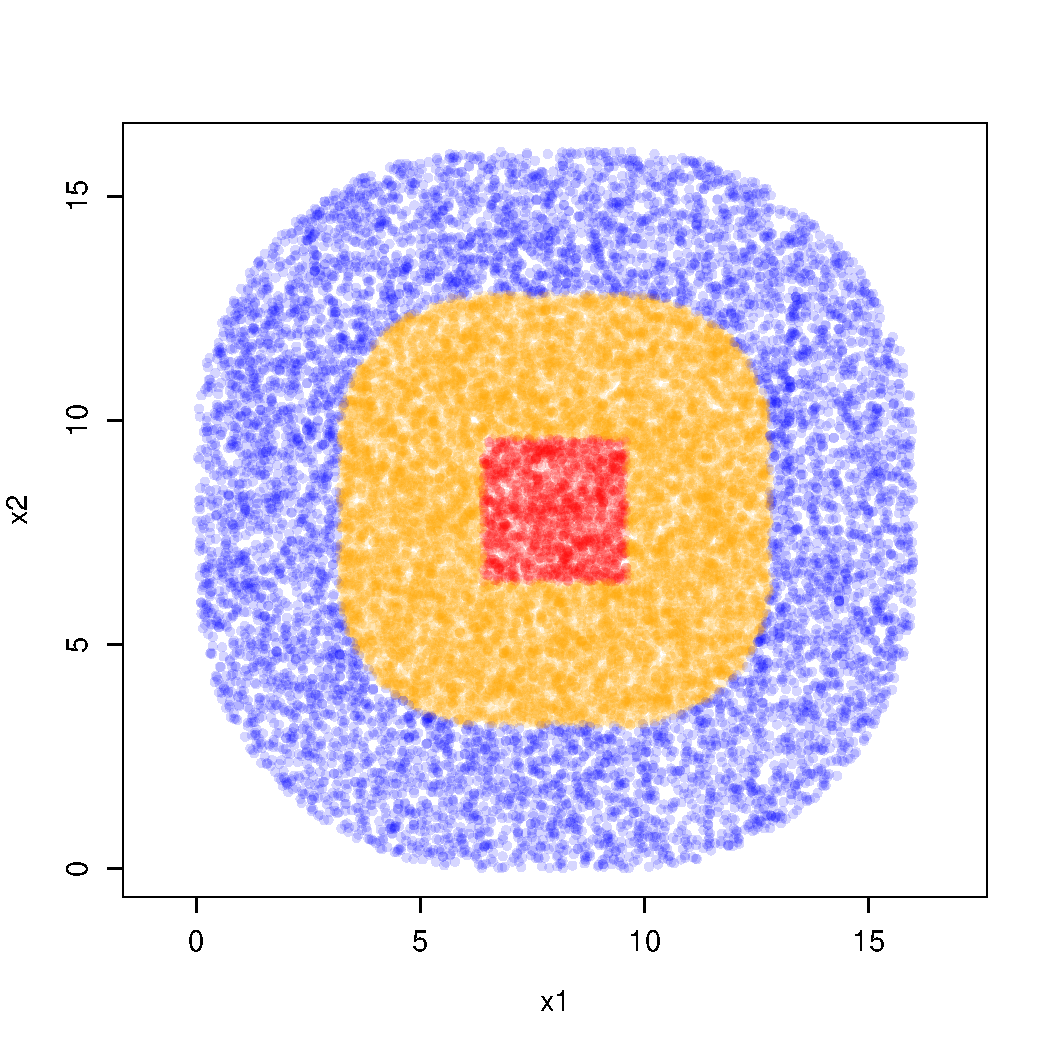
\includegraphics[width=\linewidth]{example1plots/sample2}
		\caption{}
	\end{subfigure}
	\begin{subfigure}{.33\linewidth}
		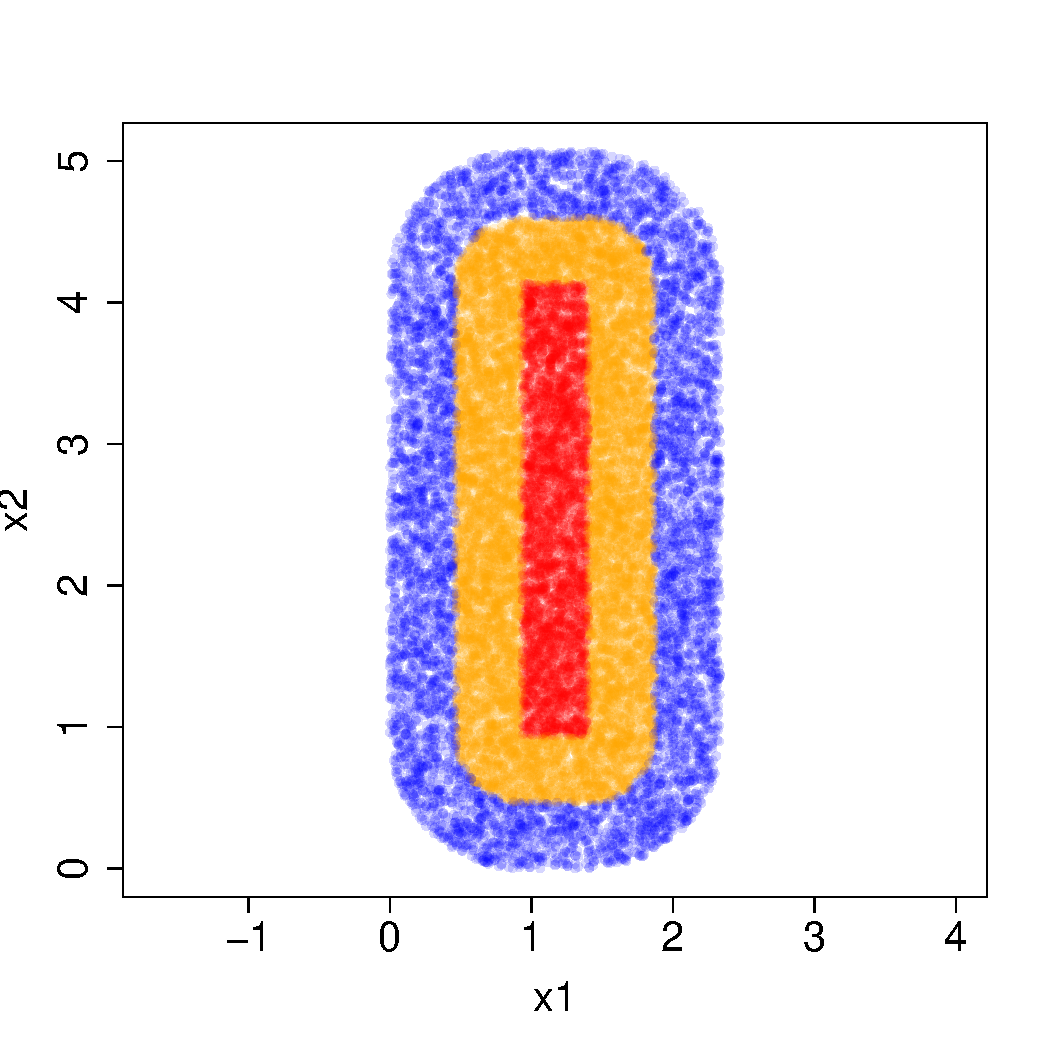
\includegraphics[width=\linewidth]{example1plots/sample1}
		\caption{}
	\end{subfigure}
	\begin{subfigure}{.33\linewidth}
		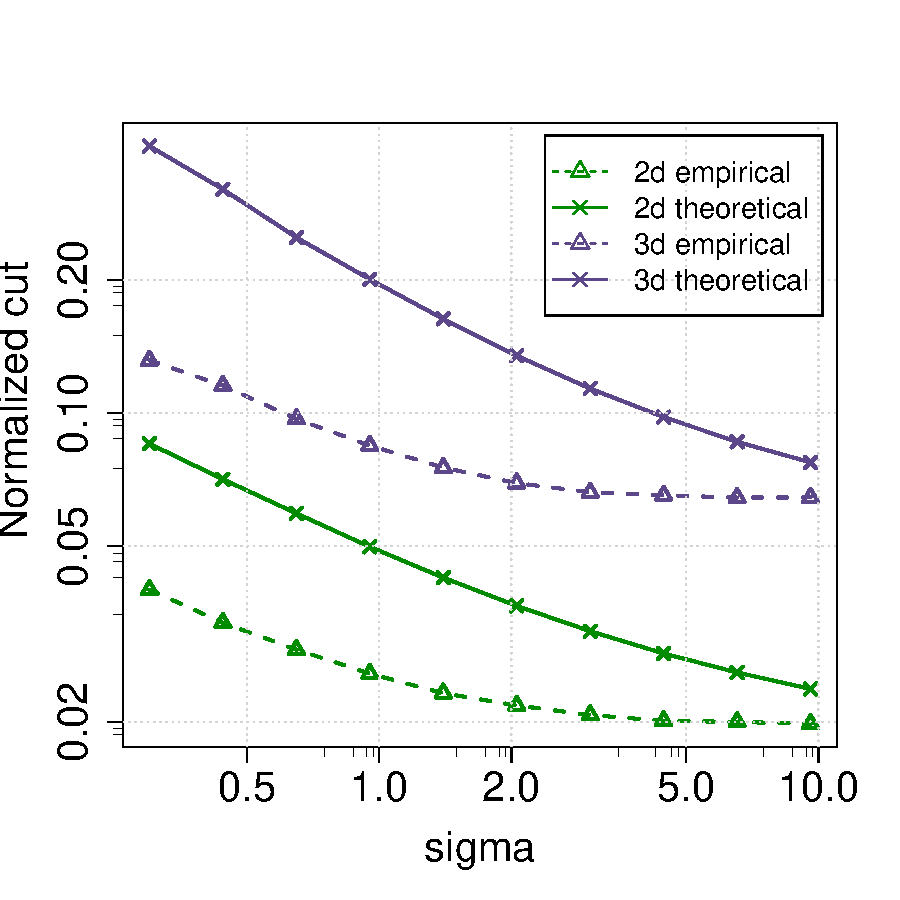
\includegraphics[width=\linewidth]{example1plots/sigma_normalized_cut_plot}
		\caption{}
	\end{subfigure}

	
	\begin{subfigure}{.33\linewidth}
		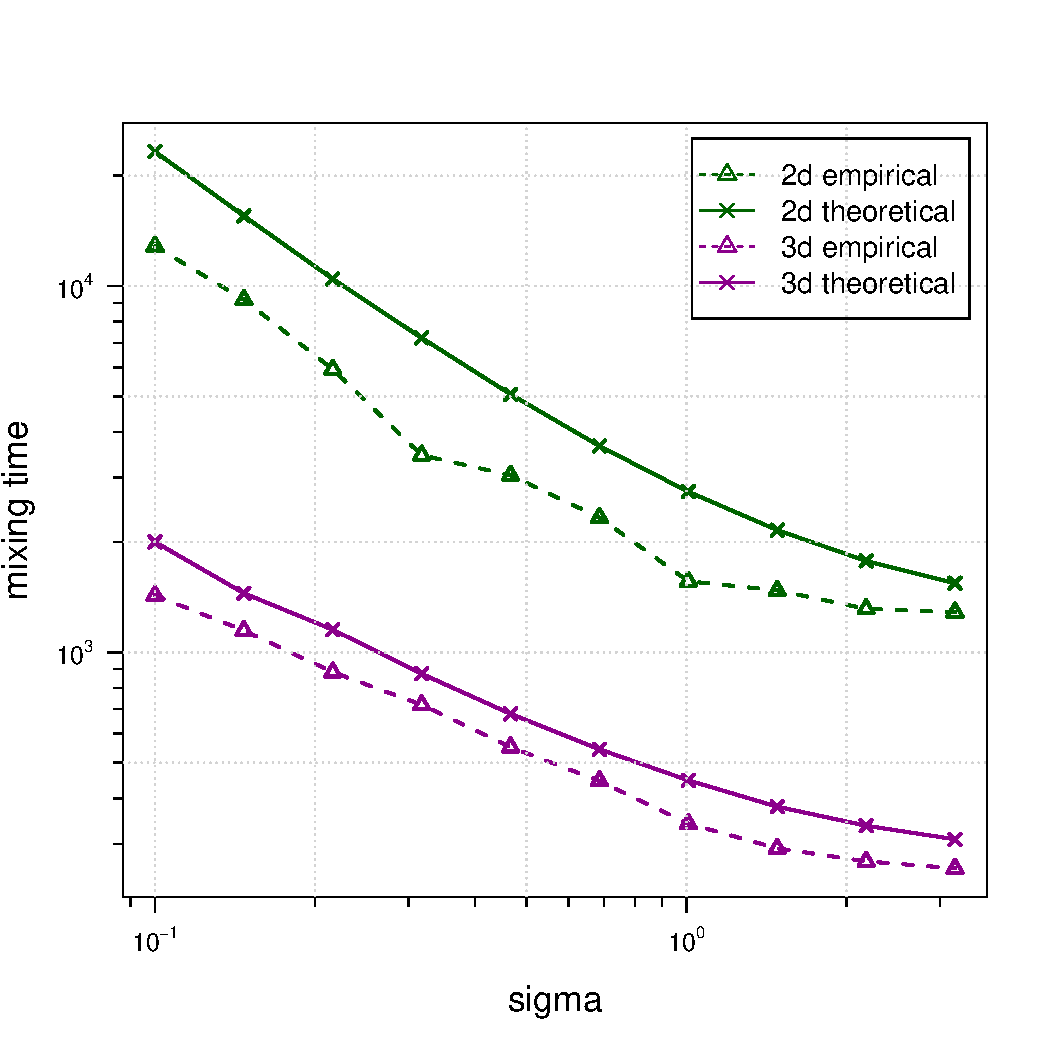
\includegraphics[width=\linewidth]{example1plots/sigma_mixing_time_plot}
		\caption{}
	\end{subfigure}
	\begin{subfigure}{.33\linewidth}
		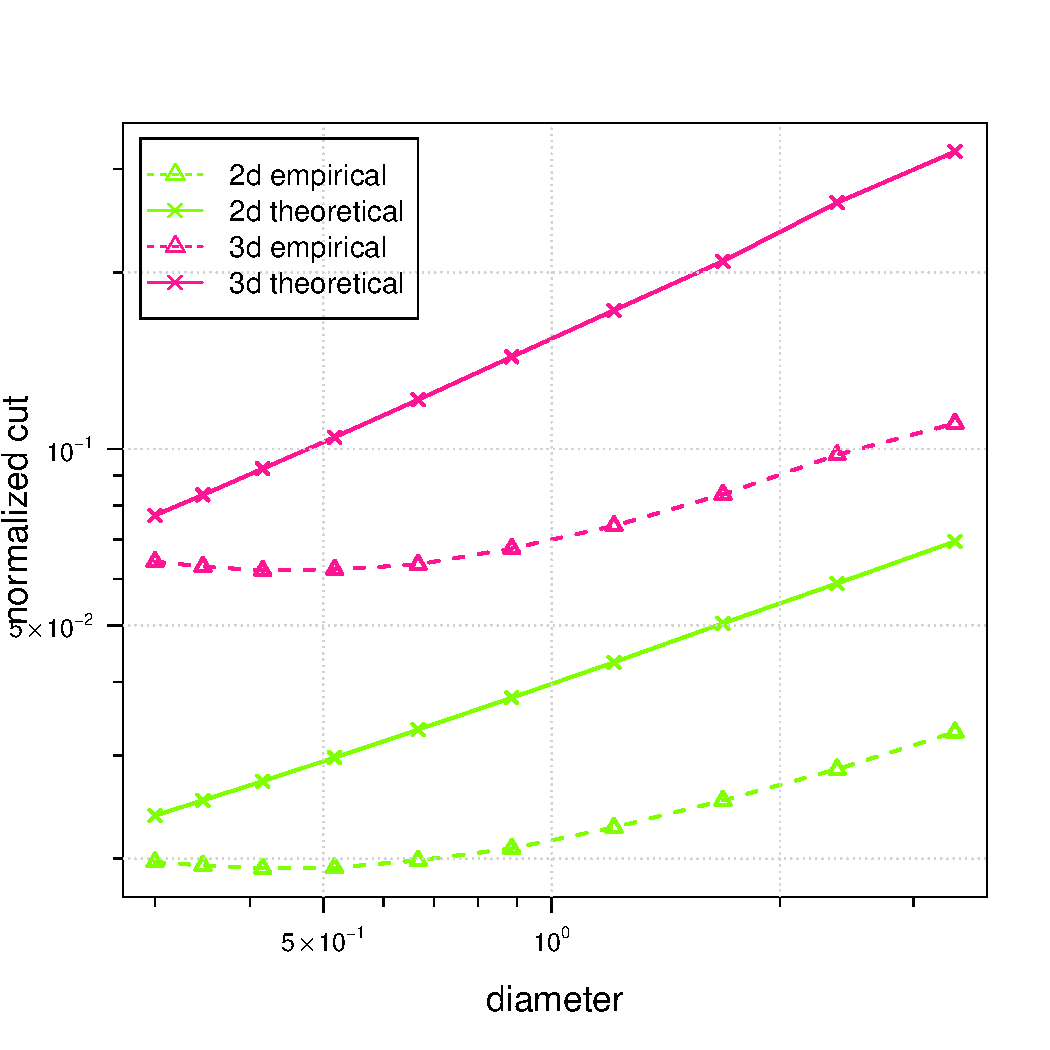
\includegraphics[width=\linewidth]{example1plots/diameter_normalized_cut_plot}
		\caption{}
	\end{subfigure}
	\begin{subfigure}{.33\linewidth}
		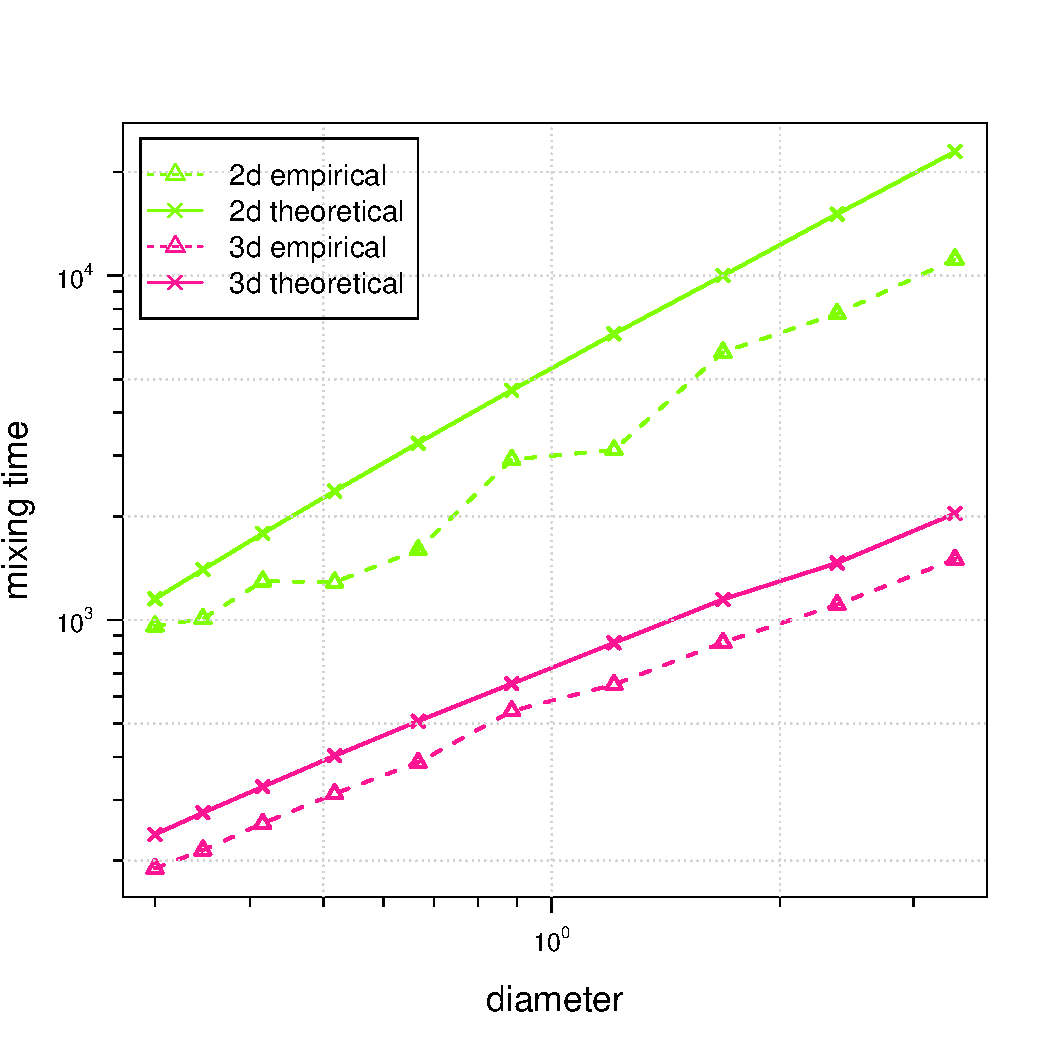
\includegraphics[width=\linewidth]{example1plots/diameter_mixing_time_plot}
		\caption{}
	\end{subfigure}
	\caption{}
	\label{fig:fig1}
	\end{adjustbox}
\end{figure}

As we do not provide any theoretical lower bounds, we validate the tightness of Theorems \ref{thm: conductance_upper_bound} and \ref{thm: inverse_mixing_time_lower_bound} via simulation.  We sample points according to the density function $q$, where for $x \in \Rd$
\begin{equation}
q(x) :=
\begin{cases}
\lambda,~ & x \in [0,\sigma] \times D^{d-1} =: \Cset, \\
\lambda - \dist(x,\Cset)\eta,~ & x \in \Csig \setminus \Cset, \\
(\lambda - \sigma \eta) - \dist(x,\Csig)^{\gamma}, & x \in (\Csig + \sigma B), \setminus \Csig \\
0,~ & \textrm{otherwise},
\end{cases}
\end{equation}
where $\lambda = \frac{150}{81} \sigma^{\gamma}$ and $\eta = \frac{15}{81} \sigma^{\gamma - 1}$. Panels $(a)$ and $(b)$ in Figure \ref{fig:fig1} show $20,000$ samples from two parameterizations of $q$. In $(a)$, $\sigma = D = 3.2$, while in $(b)$ $\sigma = .1$ and $D = 3.2$. (For both, $d = 2$).

Panels $(c) - (f)$ in Figure \ref{fig:fig1} show the change in normalized cut and mixing time, respectively, as the parameters $\sigma$ ($(c)$ and $(d)$) and $D$ ($(e)$ and $(f)$) are varied. In panels $(c)$ and $(d)$ $\sigma = .1 \cdot \sqrt{2}^j, j = 1,\ldots,10$, and $D$ is fixed at $3.2$. In panels $(e)$ and $(f)$, $D = .1 \cdot \sqrt{2}^j, j = 1,\ldots,10$ and $\sigma$ is fixed at $.1$.
For each panel, the solid lines show, up to constants \footnote{Note that we have rescaled all values of theoretical upper bounds by a constant, in order to mask the effect of large universal constants in these bounds. Therefore only comparison of slopes, rather than intercepts, is meaningful.}, the theoretical upper bound, given by Theorem \ref{thm: conductance_upper_bound} for panels $(c)$ and $(e)$ and Theorem \ref{thm: inverse_mixing_time_lower_bound} for panels $(d)$ and $(f)$. The dashed lines show the computed empirical value, averaged over $m$ trials ($m = 100$ for the normalized cut, dashed lines in panels $(c)$ and $(e)$, and $m = 20$ for the mixing time, dashed lines in panel $(d)$ and $(f)$). For each trial across all parameters, $r$, the neighborhood graph radius, is set throughout to be as small as possible such that the resulting graph is connected, for computational efficiency. Green lines correspond to dimension $d = 2$, whereas purple/pink lines correspond to $d = 3$. 

Panels $(d)$ and $(f)$ show the solid lines tracking closely to the dashed lines, in both 2 and 3 dimensions. This provides empirical evidence that the upper bound on mixing time given by Theorem \ref{thm: inverse_mixing_time_lower_bound} has the right dependency on both thickness parameter  $\sigma$ and diameter $D$.

\textcolor{red}{The story in panels $(c)$ and $(e)$ is more subtle. We note that while, broadly speaking, the trends do not appear to match, this gap between theory and empirical results is mostly due to the relationship when $\sigma \approx D$; this is the right hand side on panel $(c)$ and the left hand side on panel $(e)$. It is in these regions that the slopes of the dashed and solid lines appear most distinct. As the ratio $D/\sigma$ grows, we see the slopes of the empirical curves converging towards those predicted by theory. The takeaway message is that while the dependency in \eqref{eqn: conductance_additive_error_bound} on $\sigma$ and $D$ is loose for clusters with diameter close to thickness, it becomes tighter and tigher as $D/\sigma$ grows.}


\subsection{Empirical PPR, normalized cut, and density clustering comparison}

\begin{figure}
	\centering
	\begin{adjustbox}{minipage=\linewidth,scale=0.8}
	\begin{subfigure}{.24\linewidth}
		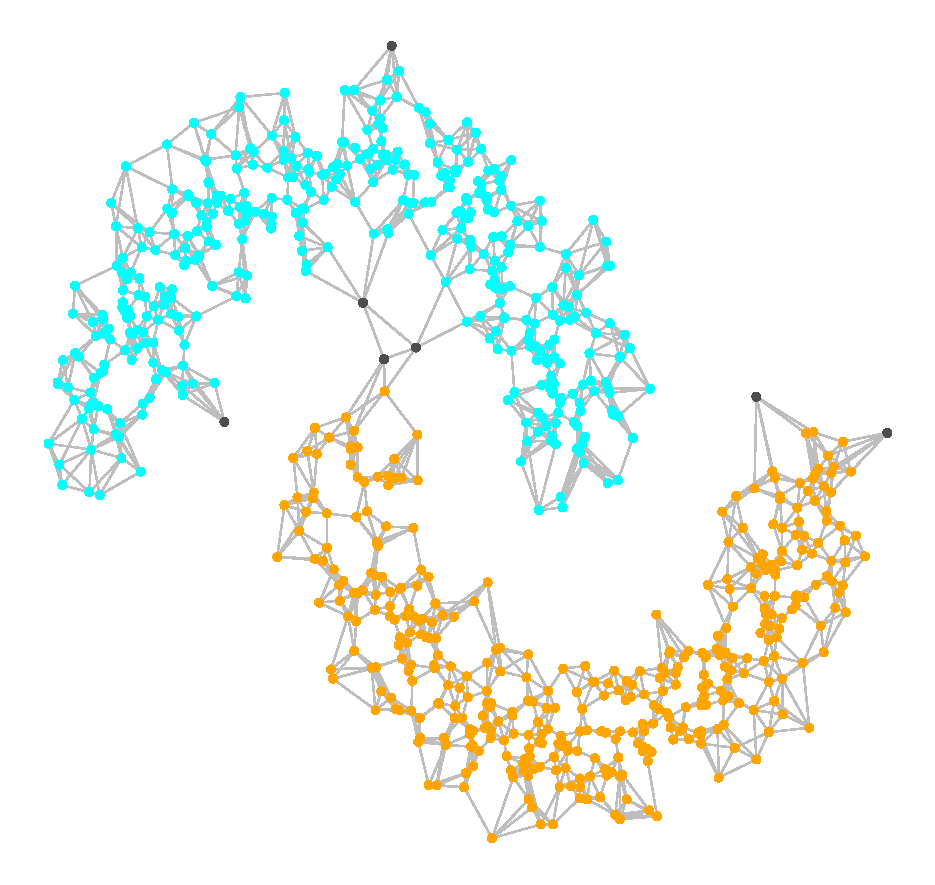
\includegraphics[width=\linewidth,scale = .5]{example2plots/row1_true_density_cluster}
		\caption{}
	\end{subfigure}
	\begin{subfigure}{.24\linewidth}
		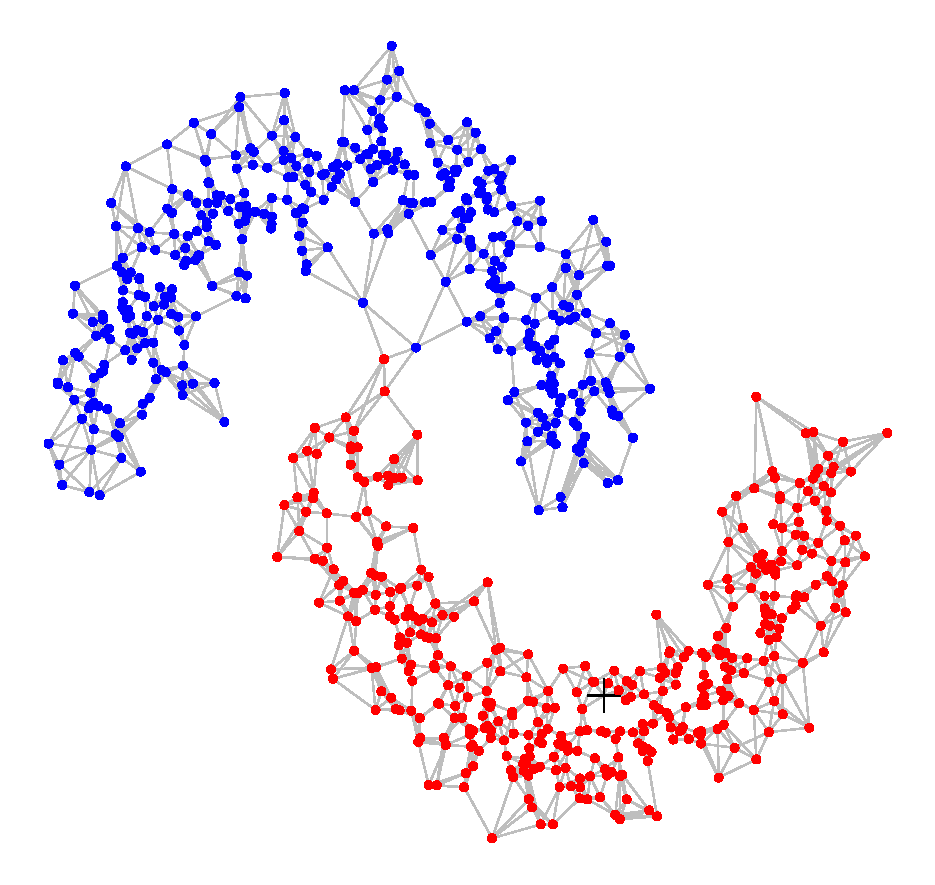
\includegraphics[width=\linewidth]{example2plots/row1_ppr_cluster}
		\caption{}
	\end{subfigure}
	\begin{subfigure}{.24\linewidth}
		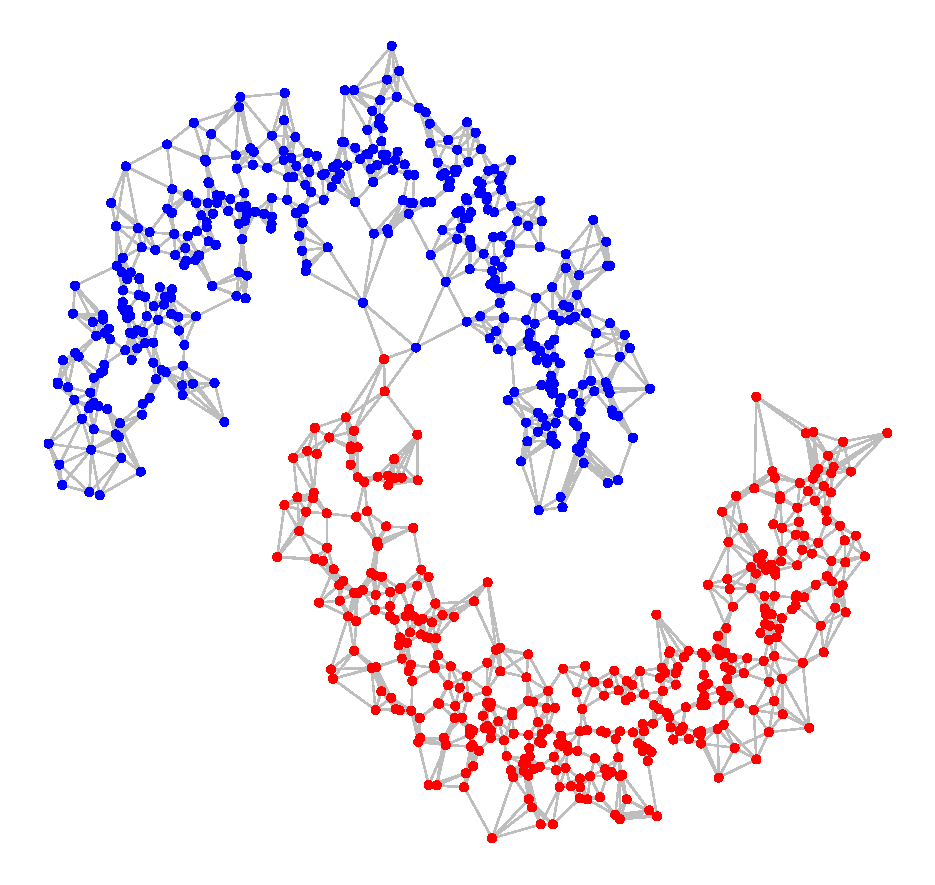
\includegraphics[width=\linewidth]{example2plots/row1_conductance_cluster}
		\caption{}
	\end{subfigure}
	\begin{subfigure}{.24\linewidth}
		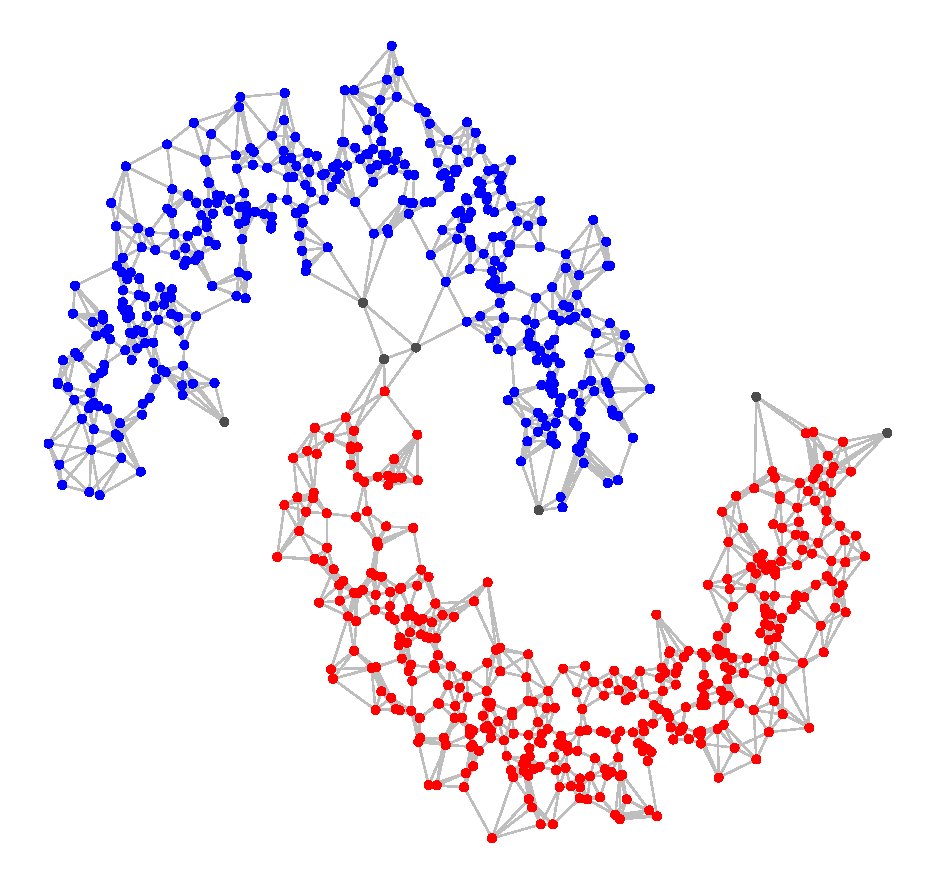
\includegraphics[width=\linewidth]{example2plots/row1_density_cluster}
		\caption{}
	\end{subfigure}
	
	\begin{subfigure}{.24\linewidth}
		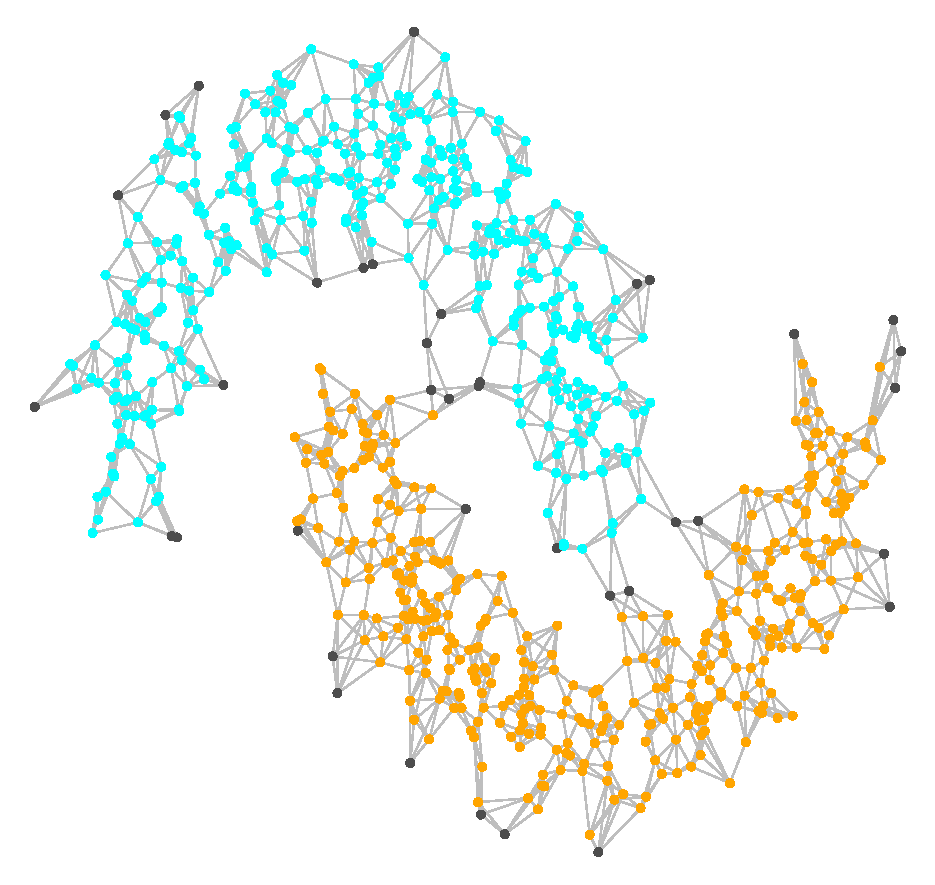
\includegraphics[width=\linewidth]{example2plots/row2_true_density_cluster}
		\caption{}
	\end{subfigure}
	\begin{subfigure}{.24\linewidth}
		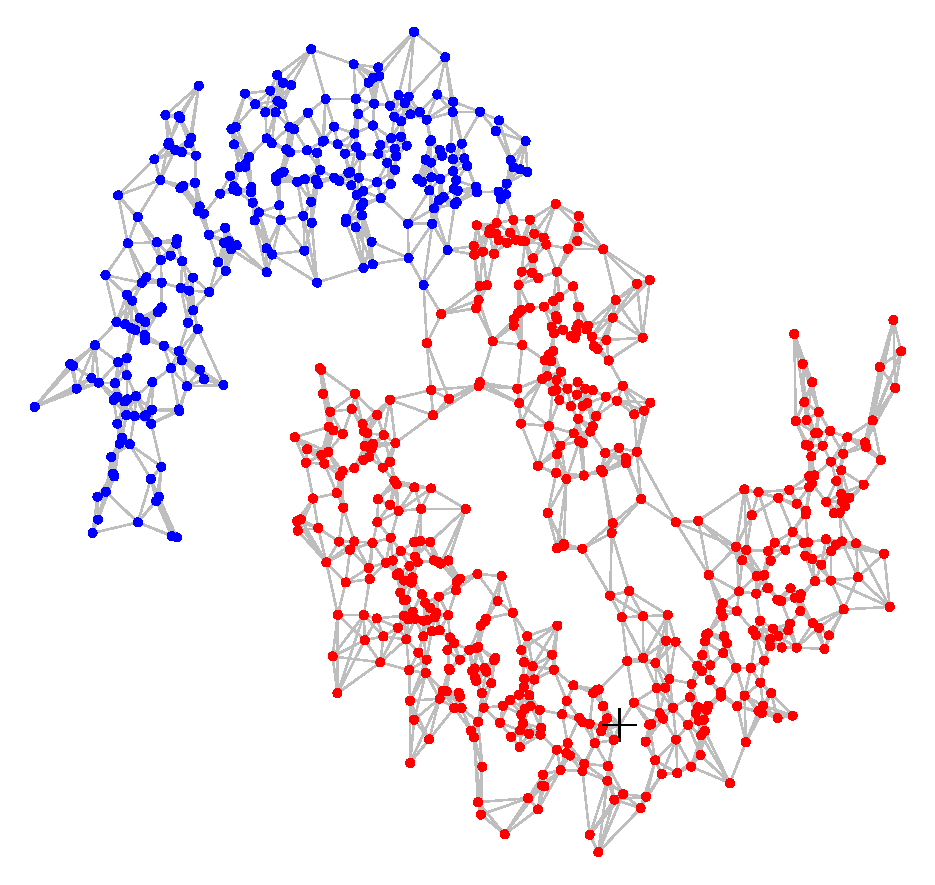
\includegraphics[width=\linewidth]{example2plots/row2_ppr_cluster}
		\caption{}
	\end{subfigure}
	\begin{subfigure}{.24\linewidth}
		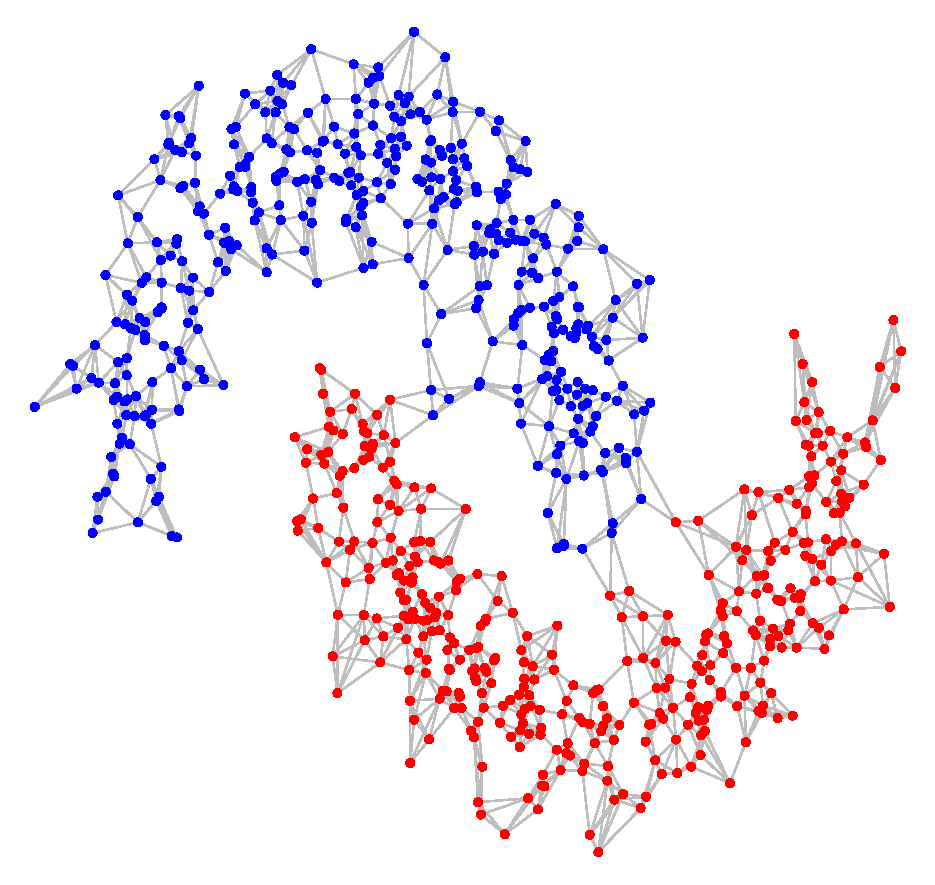
\includegraphics[width=\linewidth]{example2plots/row2_conductance_cluster}
		\caption{}
	\end{subfigure}
	\begin{subfigure}{.24\linewidth}
		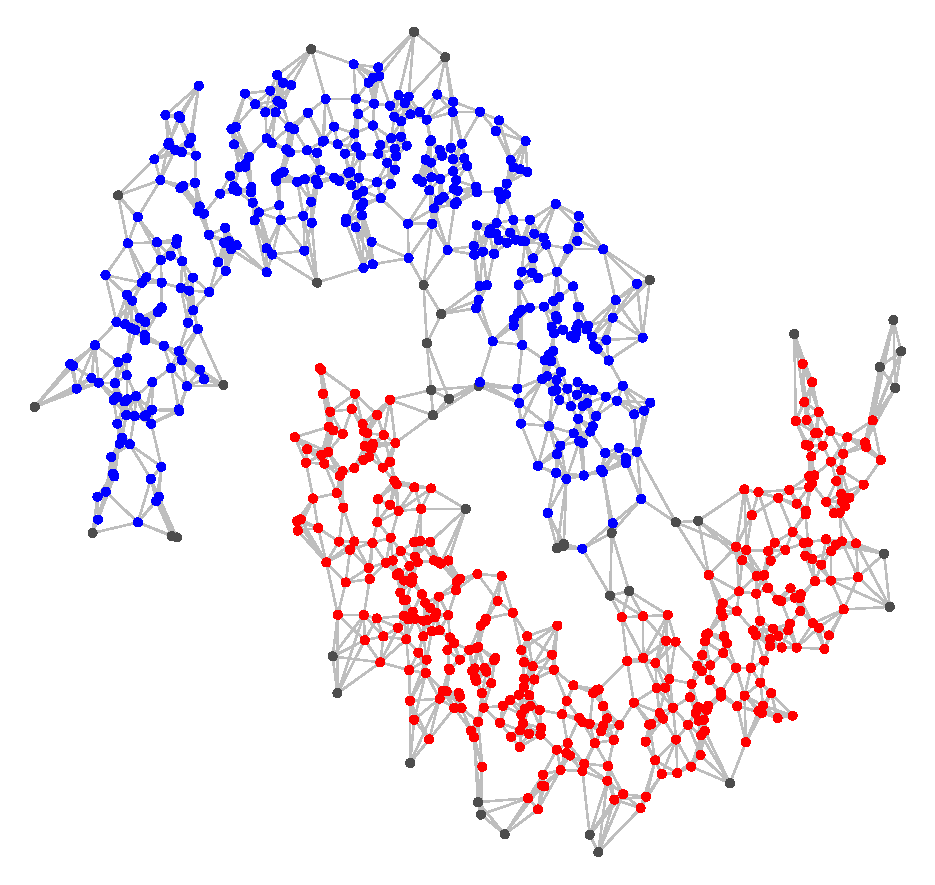
\includegraphics[width=\linewidth]{example2plots/row2_density_cluster}
		\caption{}
	\end{subfigure}
	
	\begin{subfigure}{.24\linewidth}
		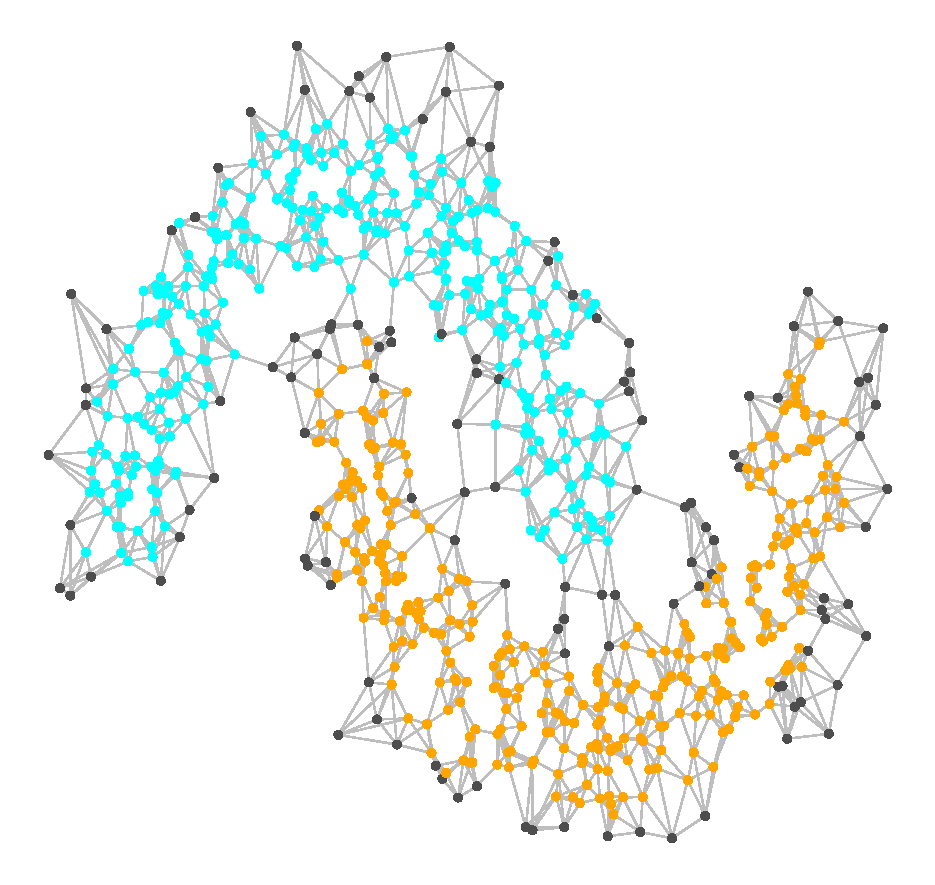
\includegraphics[width=\linewidth]{example2plots/row3_true_density_cluster}
		\caption{}
	\end{subfigure}
	\begin{subfigure}{.24\linewidth}
		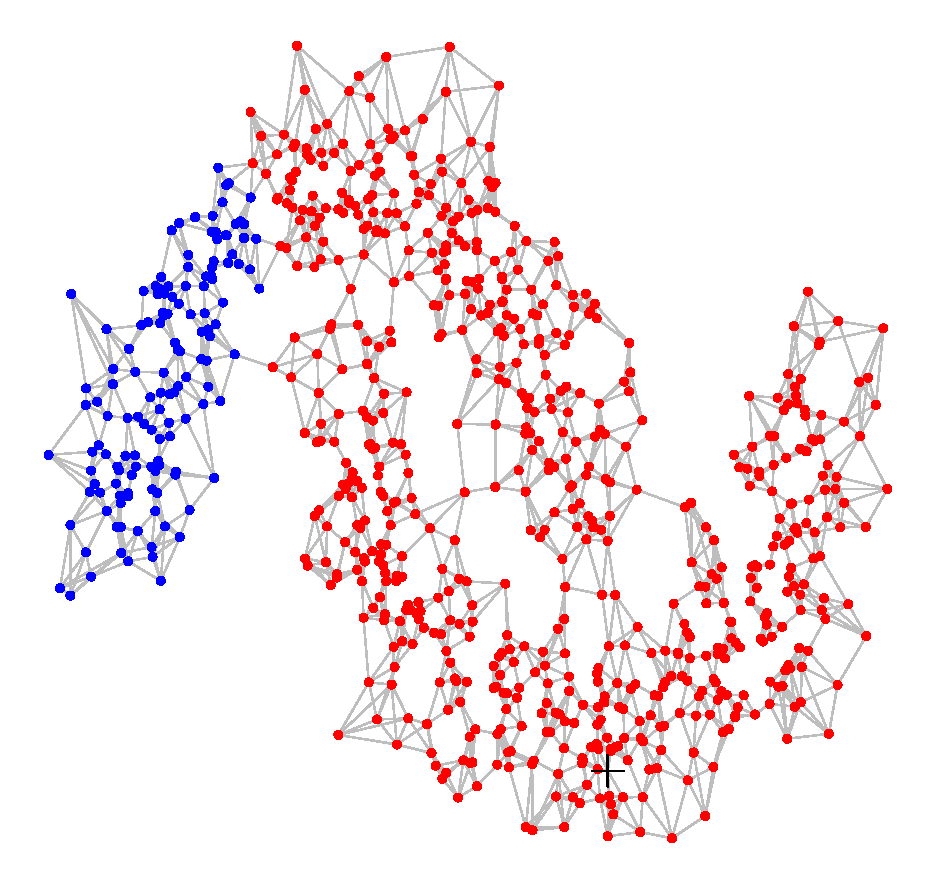
\includegraphics[width=\linewidth]{example2plots/row3_ppr_cluster}
		\caption{}
	\end{subfigure}
	\begin{subfigure}{.24\linewidth}
		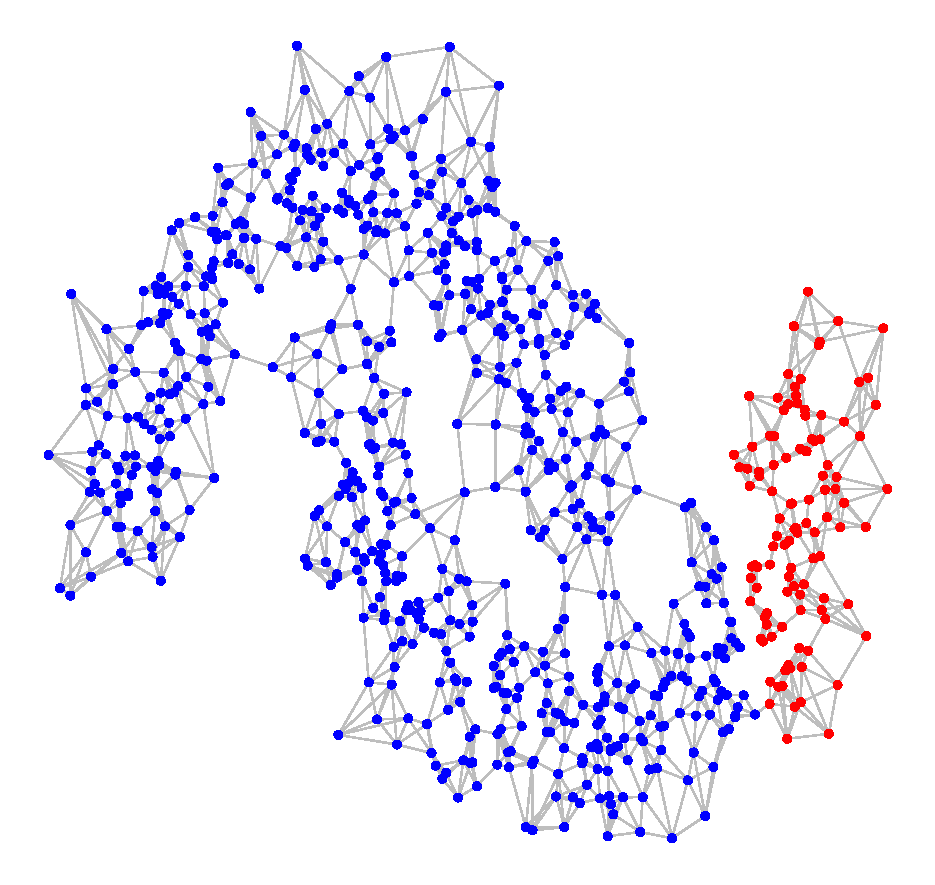
\includegraphics[width=\linewidth]{example2plots/row3_conductance_cluster}
		\caption{}
	\end{subfigure}
	\begin{subfigure}{.24\linewidth}
		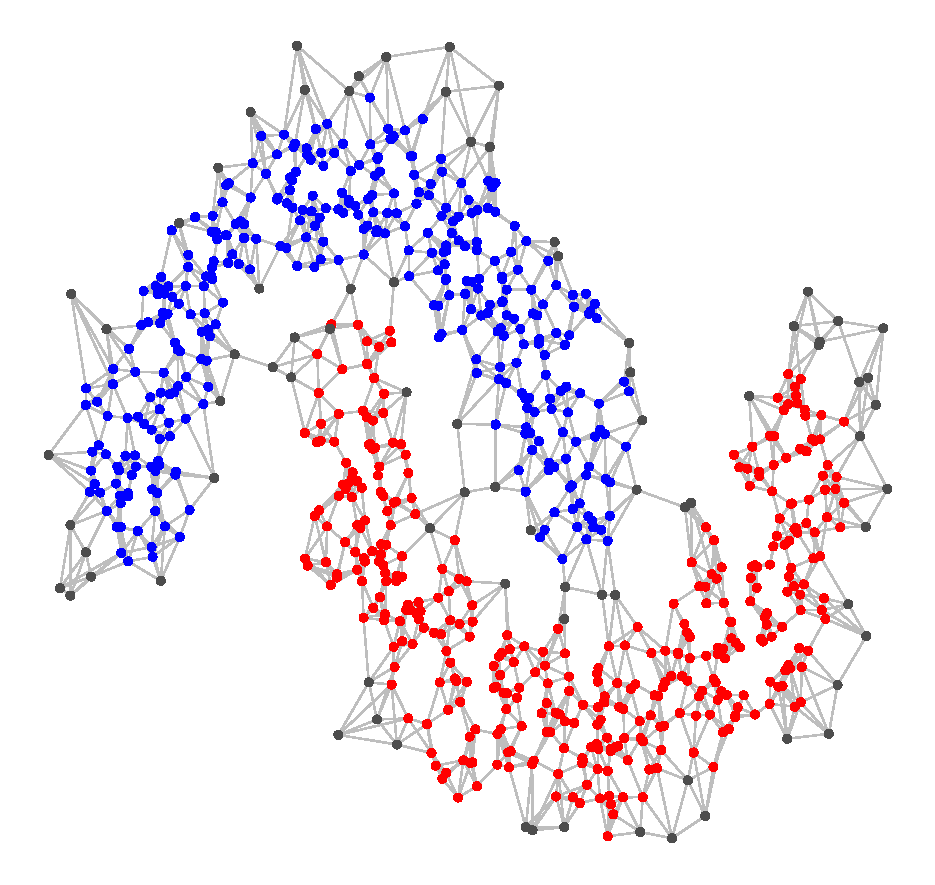
\includegraphics[width=\linewidth]{example2plots/row3_density_cluster}
		\caption{}
	\end{subfigure}
	
	\begin{subfigure}{.24\linewidth}
		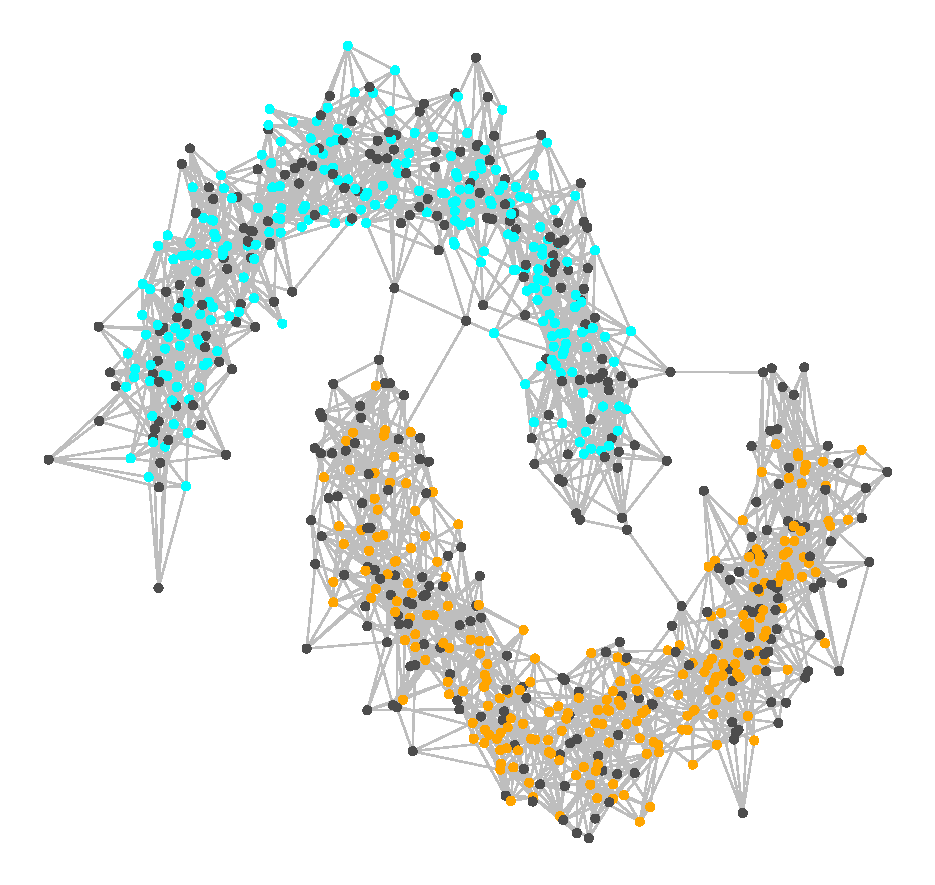
\includegraphics[width=\linewidth]{example2plots/row4_true_density_cluster}
		\caption{}
	\end{subfigure}
	\begin{subfigure}{.24\linewidth}
		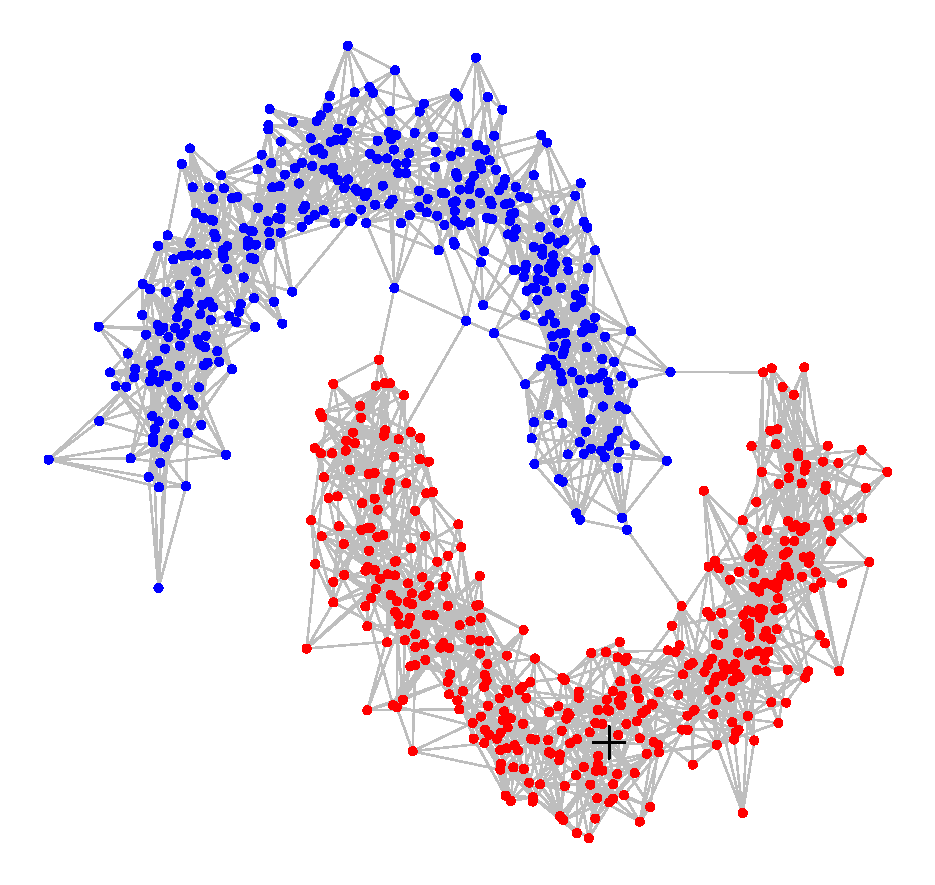
\includegraphics[width=\linewidth]{example2plots/row4_ppr_cluster}
		\caption{}
	\end{subfigure}
	\begin{subfigure}{.24\linewidth}
		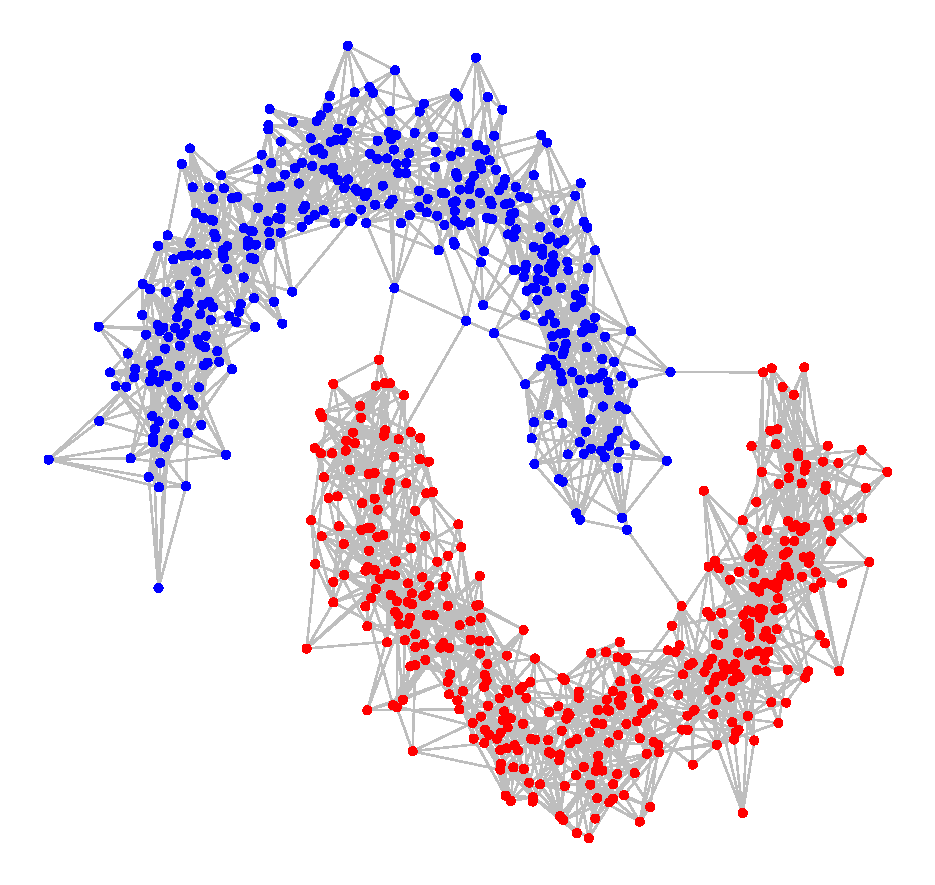
\includegraphics[width=\linewidth]{example2plots/row4_conductance_cluster}
		\caption{}
	\end{subfigure}
	\begin{subfigure}{.24\linewidth}
		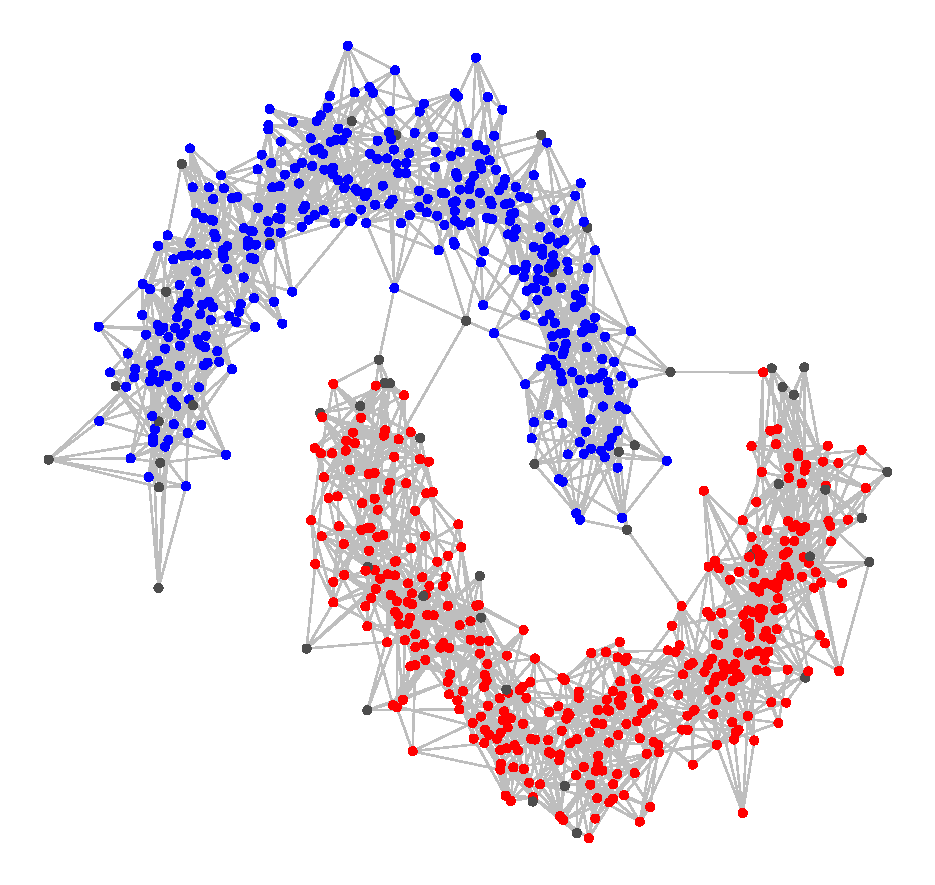
\includegraphics[width=\linewidth]{example2plots/row4_density_cluster}
		\caption{}
	\end{subfigure}
	\caption{True density (column 1), \pprspace (column 2), normalized cut (column 3) and estimated density (column 4) clusters for 4 different simulated data sets. Seed node for \pprspace denoted by a black cross.}
	\label{fig:fig2}
	\end{adjustbox}
\end{figure}

To drive home the main implications of Theorem \ref{thm: ppr_cluster}, we show the behavior of \pprspace, normalized cut, and the density clustering algorithm of \citep{chaudhuri2010} on (a variant of) the famous 'two moons' dataset, considered a prototypical success story for spectral clustering algorithms. To form each of the four rows in Figure \ref{fig:fig2}, 800 points are independently sampled following a 'two moons plus Gaussian noise model'. Formally, the (respective) generative models for the data are
\begin{align}
Z & \sim \textrm{Bern}(1/2), \theta \sim \textrm{Unif}(0, \pi) \\
X(Z,\theta) & = 
\begin{cases}
\mu_1 + (r \cos(\theta), r \sin(\theta)) + \sigma \epsilon,~ & \text{if}~ Z = 1 \\
\mu_2 + (r \cos(\theta), - r \sin(\theta)) + \sigma \epsilon,~ & \text{if}~ Z = 0
\end{cases}
\end{align}

where 
\begin{align*}
\mu_1 & = (-.5, 0),~ \mu_2 = (0,0),~ \epsilon \sim N(0, I_2) \tag{row 1} \\
\mu_1 & = (-.5, -.07),~ \mu_2 = (0,.07),~ \epsilon \sim N(0, I_2) \tag{row 2} \\
\mu_1 & = (-.5, -.125),~ \mu_2 = (0,.125),~ \epsilon \sim N(0, I_2) \tag{row 3} \\
\mu_1 & = (-.5, -.025),~ \mu_2 = (0,.025),~ \epsilon \sim N(0, I_{10}) \tag{row 4}
\end{align*}
for $I_d$ the $d \times d$ identity matrix. The first column consists of the empirical density clusters $C_n$ and $C_n'$ for a particular threshold $\lambda$ of the density function; the second column shows the ~\pprspace plus minimum normalized sweep cut cluster, with hyperparameter $\alpha$ and all sweep cuts considered; the third column shows the global minimum normalized cut, computed according to the algorithm of \textcolor{red}{Bressson et al. 2012}; and the last column shows a cut of the cluster tree estimator of \textcolor{red}{Chaudhuri Dasgupta}

Rows 1-3 show the degrading ability of \pprspace to recover density clusters as the two moons become less salient. In the first row, the normalized cut conforms to the density cluster, and \pprspace recovers both. In the second row, the normalized cut still conforms to the density cluster, but because the internal connectivity of the lower moon is low, \pprspace fails to recover the normalized cut. In the third row, the moons have such low saliency that even the normalized cut fails to recover the lower moon; we also see from $(k)$ that \pprspace does not somehow save us in this situation. Note that this is not a function of the finite sample: the 4th column shows us that the Chaudhuri Dasgupta cluster tree estimator can be recover the true density cluster.

The fourth row illustrates the effect of dimension. The gray dots in $(m)$ (as in $(a), (e)$ and $(i)$ are observations in low-density regions. While the \pprspace sweep cut $(n)$ has relatively high symmetric set difference with the chosen density cut, it still recovers $C_n$ in the sense of Definition \textcolor{red}{1}.


\section{Discussion}
\label{sec: discussion}
For a clustering algorithm and a given object (such as a graph or set of points), there are an almost limitless number of ways to define what the 'right' clustering is. We have considered a few such ways -- density level sets, and the bicriteria of normalized cut, inverse mixing time -- and shown that under the right conditions, the latter agree with the former, with resulting algorithmic consequences.

There are still many directions worth pursuing in this area. Concretely, we might wish to generalize our results to hold over a wider range of kernel functions, and hyperparameter inputs to the \pprspace algorithm. More broadly, we do not provide any sort of theoretical lower bound, although we give empirical evidence in Figures \ref{fig: graphic_1} and \ref{fig: graphic_2} that poorly conditioned density clusters are not consistently estimated by \pprspace.

The initial motivation for this article was based on the intuition that density level sets, in the right conditions, will have small normalized cut. As a result, algorithms with normalized cut based guarantees (such as \pprspace) seemed likely to have density cluster recovery guarantees as well. However, the second-order behavior of \pprspace when failing to recover the conductance cut is also of interest. Are there situations when the conductance cut and density cut differ, yet \pprspace still recovers the latter? This is an open question.

\clearpage

\bibliographystyle{plainnat}
\bibliography{../local_spectral_bibliography}



\end{document}